\documentclass[english]{beamer} %,handout
\usepackage{amsmath}
\usepackage{graphicx}
\usepackage[cjk,hangul,usecjkt1font]{kotex}

\makeatletter

\usepackage{listings}
\setbeamertemplate{footline}[frame number]
\setbeamercovered{transparent}

\usecolortheme{kesl}

\usepackage[absolute,overlay]{textpos}
\setlength{\TPHorizModule}{\paperwidth}
\setlength{\TPVertModule}{\paperheight}
\textblockorigin{0mm}{0mm}
 
\usepackage{babel}
\beamertemplatenavigationsymbolsempty
\usepackage{verbatim}
\begin{document}

\title[Memory Scalability]{
경량 로그 기반 지연 업데이트 기법을 활용한 리눅스 커널 확장성 향상 \\
\small{A Lightweight Log-based Deferred Update
for \\Linux Kernel Scalability}}

\author{Joohyun Kyong}
\institute[Kookmin University]
{
  School of Computer Science\\
  Kookmin University\\
  Thesis advisor: Sung-soo Lim
}

\setbeamercovered{dynamic} 
%TODO Audit Words, reduce

\begin{frame}
  \titlepage
\end{frame}

\begin{frame}{40 Years of Microprocessor Trend Data}
\pgfdeclareimage[width=\paperwidth]{cpu_1}{.//slides/cpu_1}
\begin{textblock}{1}(0,0)
\pgfuseimage<+->{cpu_1}
\end{textblock}
\end{frame}


\begin{frame}{40 Years of Microprocessor Trend Data}
\pgfdeclareimage[width=\paperwidth]{cpu_2}{.//slides/cpu_2}
\begin{textblock}{1}(0,0)
\pgfuseimage<+->{cpu_2}
\end{textblock}
\end{frame}

\begin{frame}{40 Years of Microprocessor Trend Data}
\pgfdeclareimage[width=\paperwidth]{cpu_3}{.//slides/cpu_3}
\begin{textblock}{1}(0,0)
\pgfuseimage<+->{cpu_3}
\end{textblock}
\end{frame}


\begin{frame}{40 Years of Microprocessor Trend Data}
\pgfdeclareimage[width=\paperwidth]{cpu_4}{.//slides/cpu_4}
\begin{textblock}{1}(0,0)
\pgfuseimage<+->{cpu_4}
\end{textblock}
\end{frame}


\begin{frame}{OS Kernel Scalability History}
\begin{center}
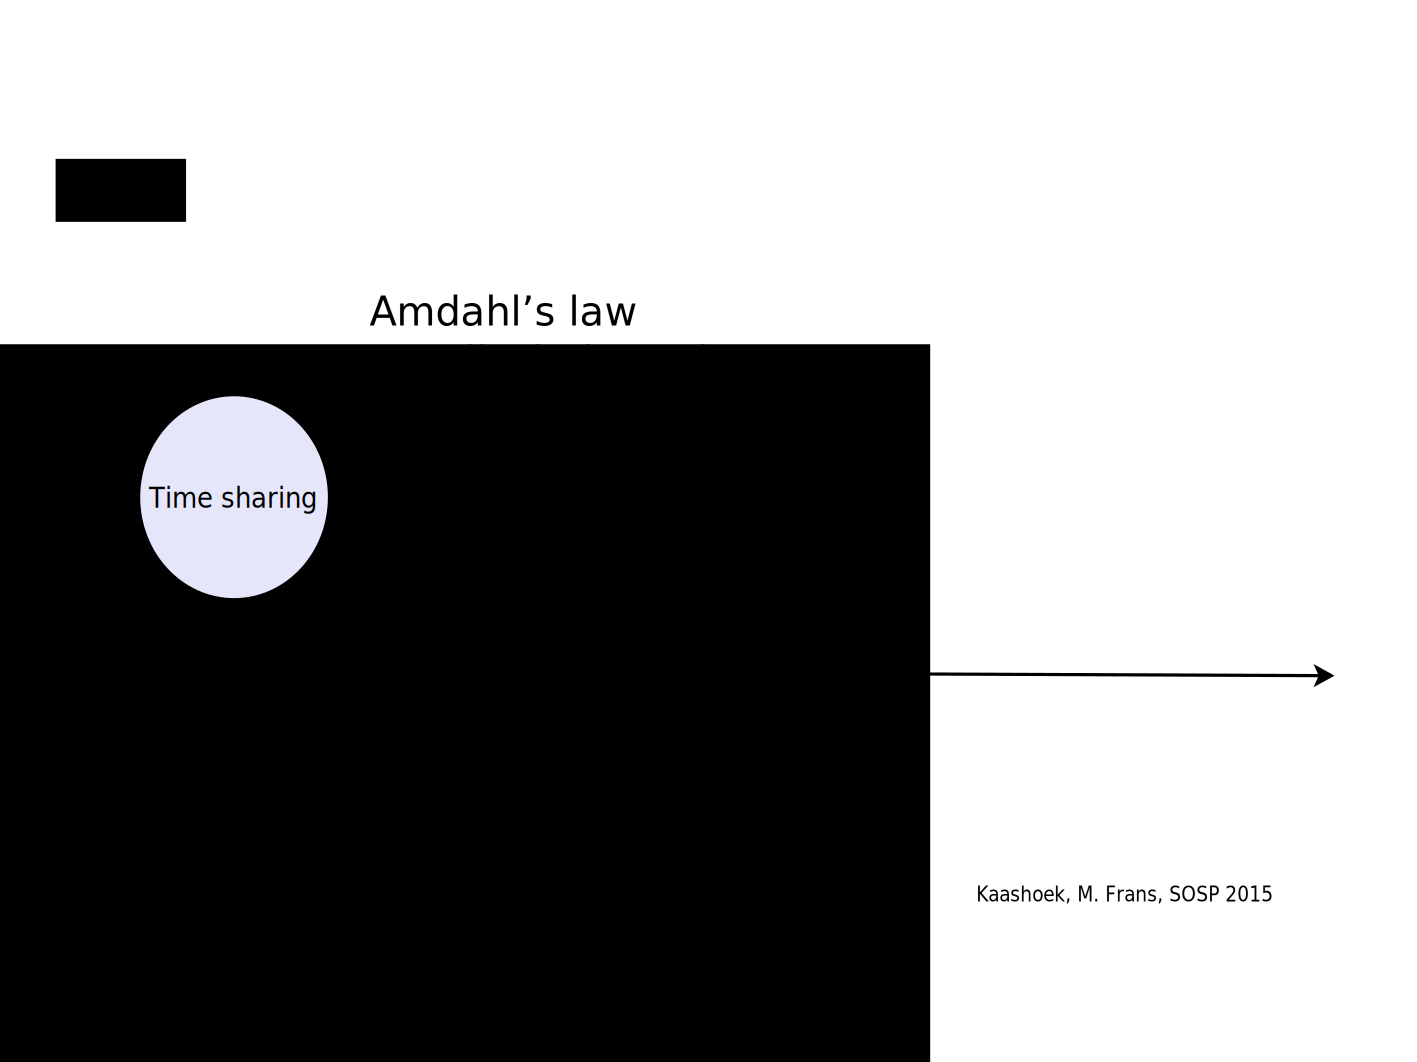
\includegraphics[scale=0.3]{fig/history_old_60s}
\end{center}
\end{frame}


\begin{frame}{OS Kernel Scalability History}
\begin{center}
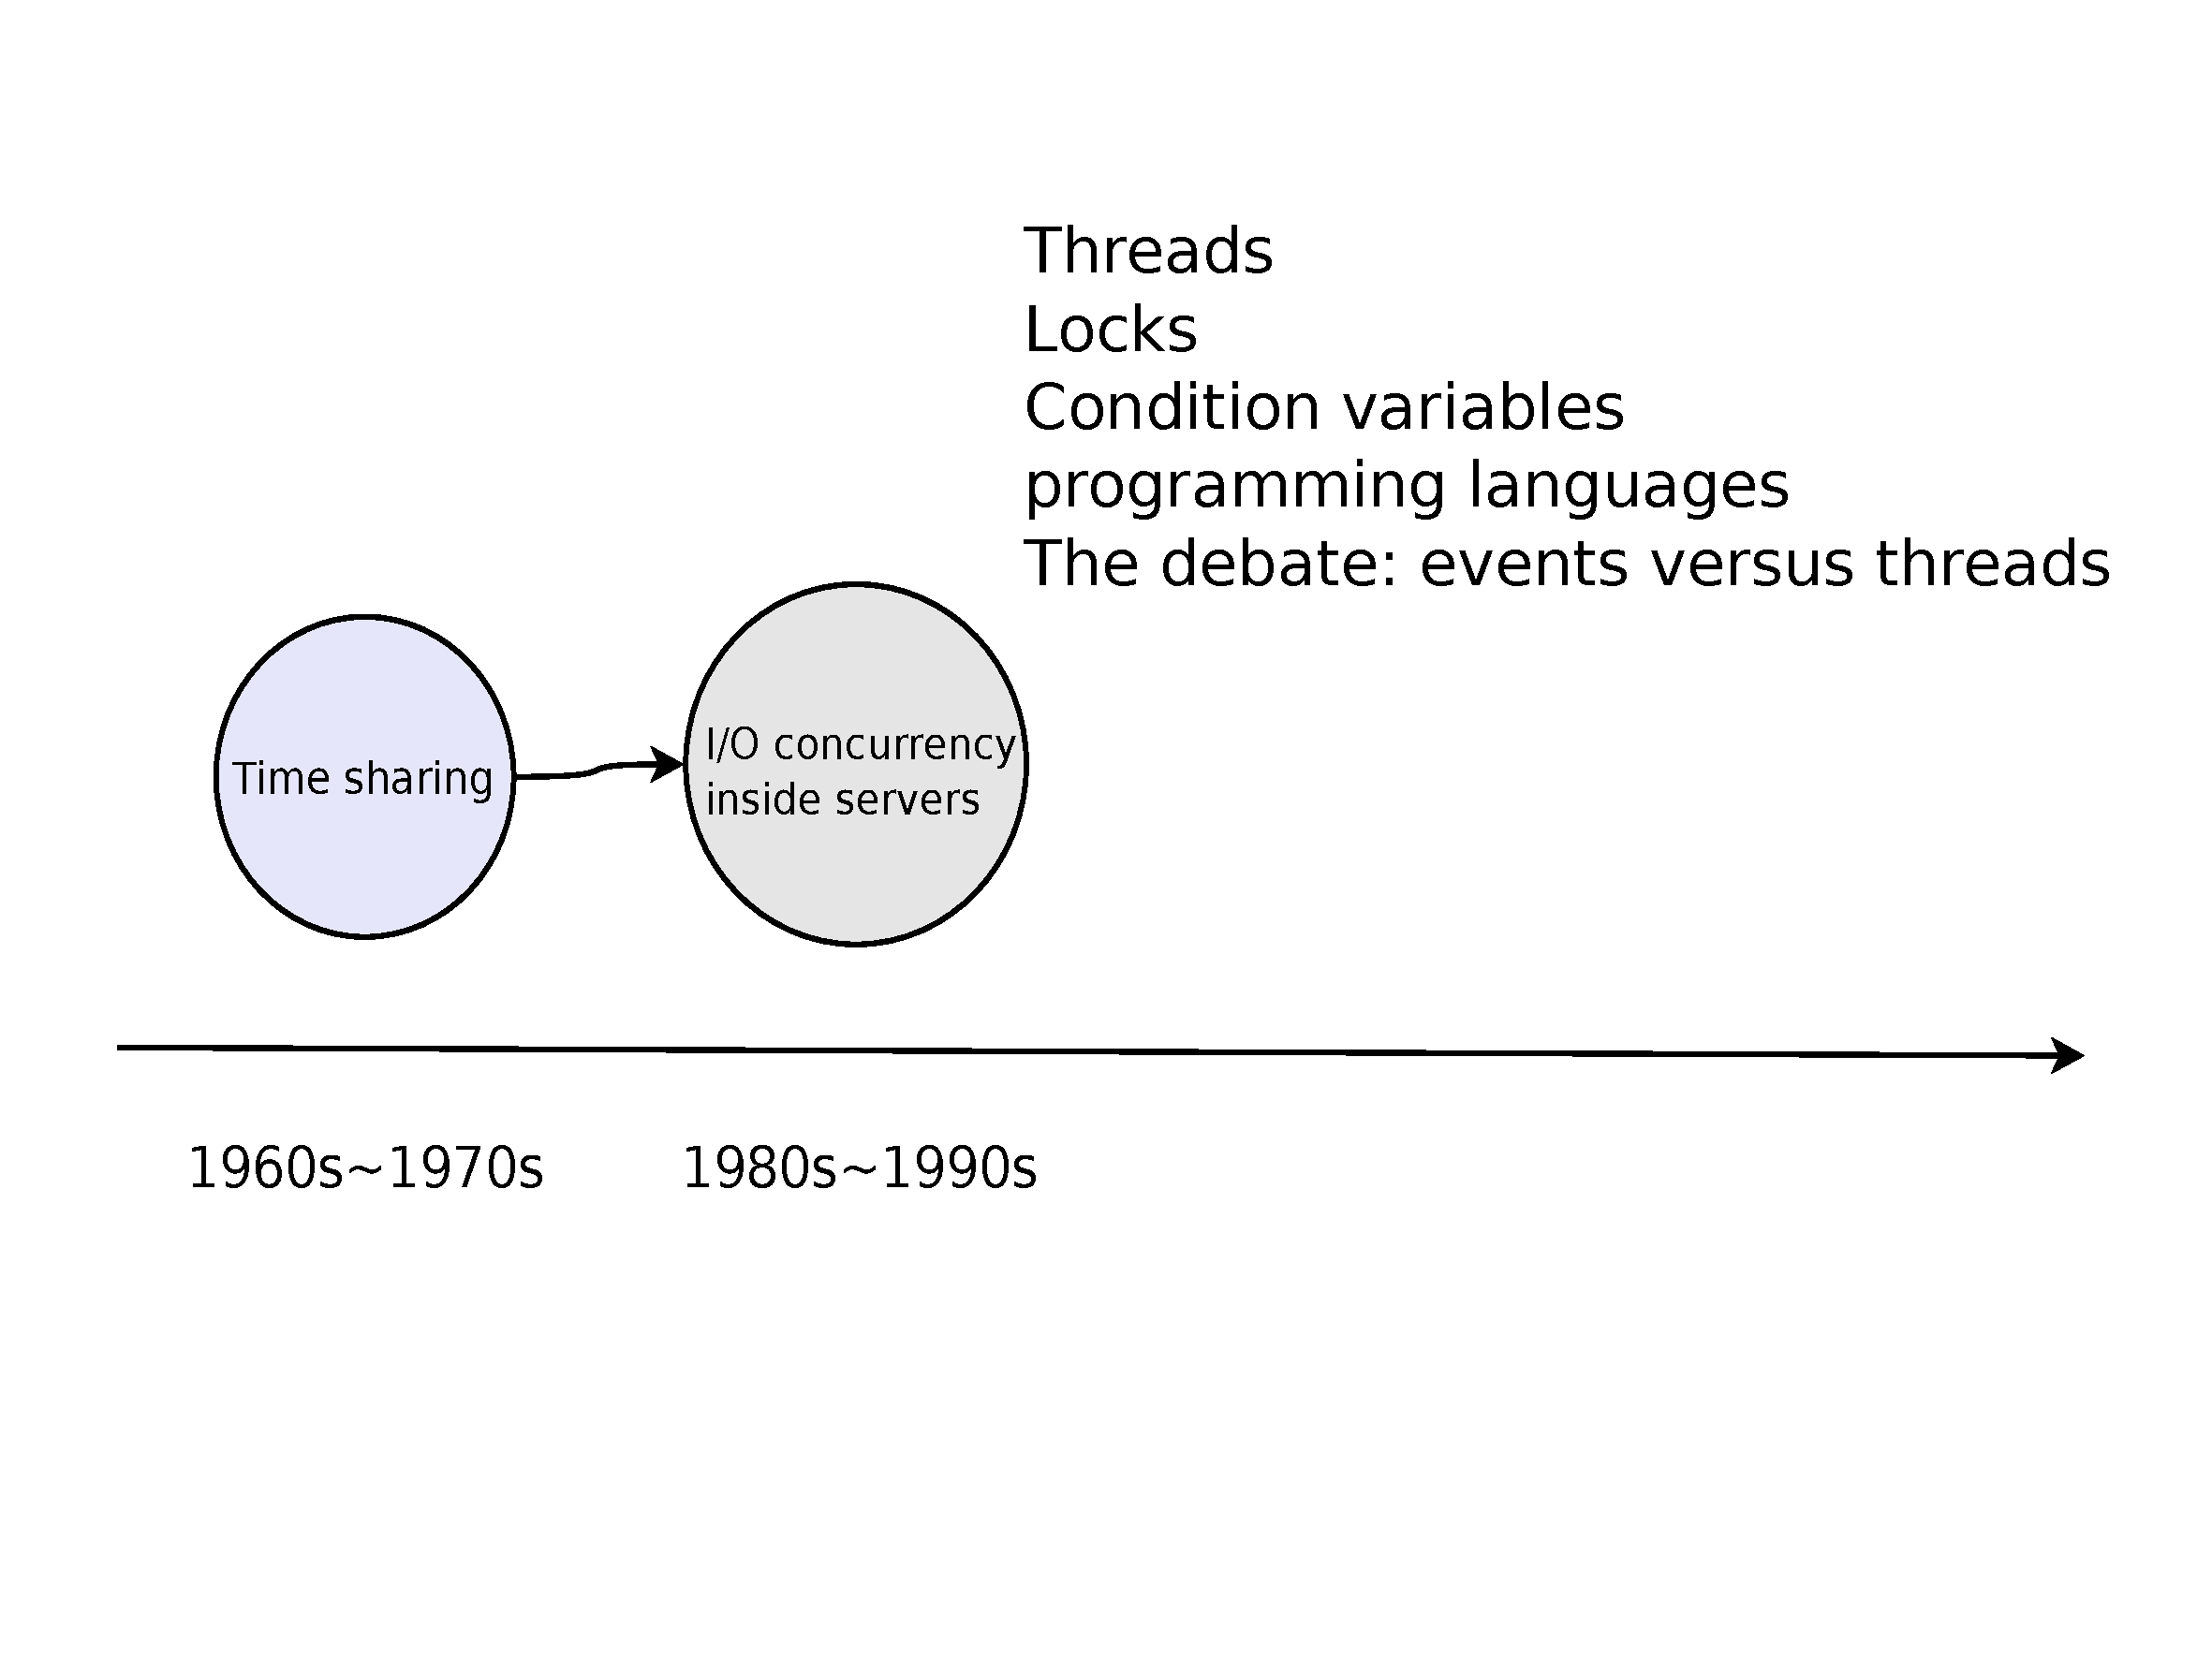
\includegraphics[scale=0.3]{fig/history_old_80s}
\end{center}
\end{frame}


\begin{frame}{OS Kernel Scalability History}
\begin{center}
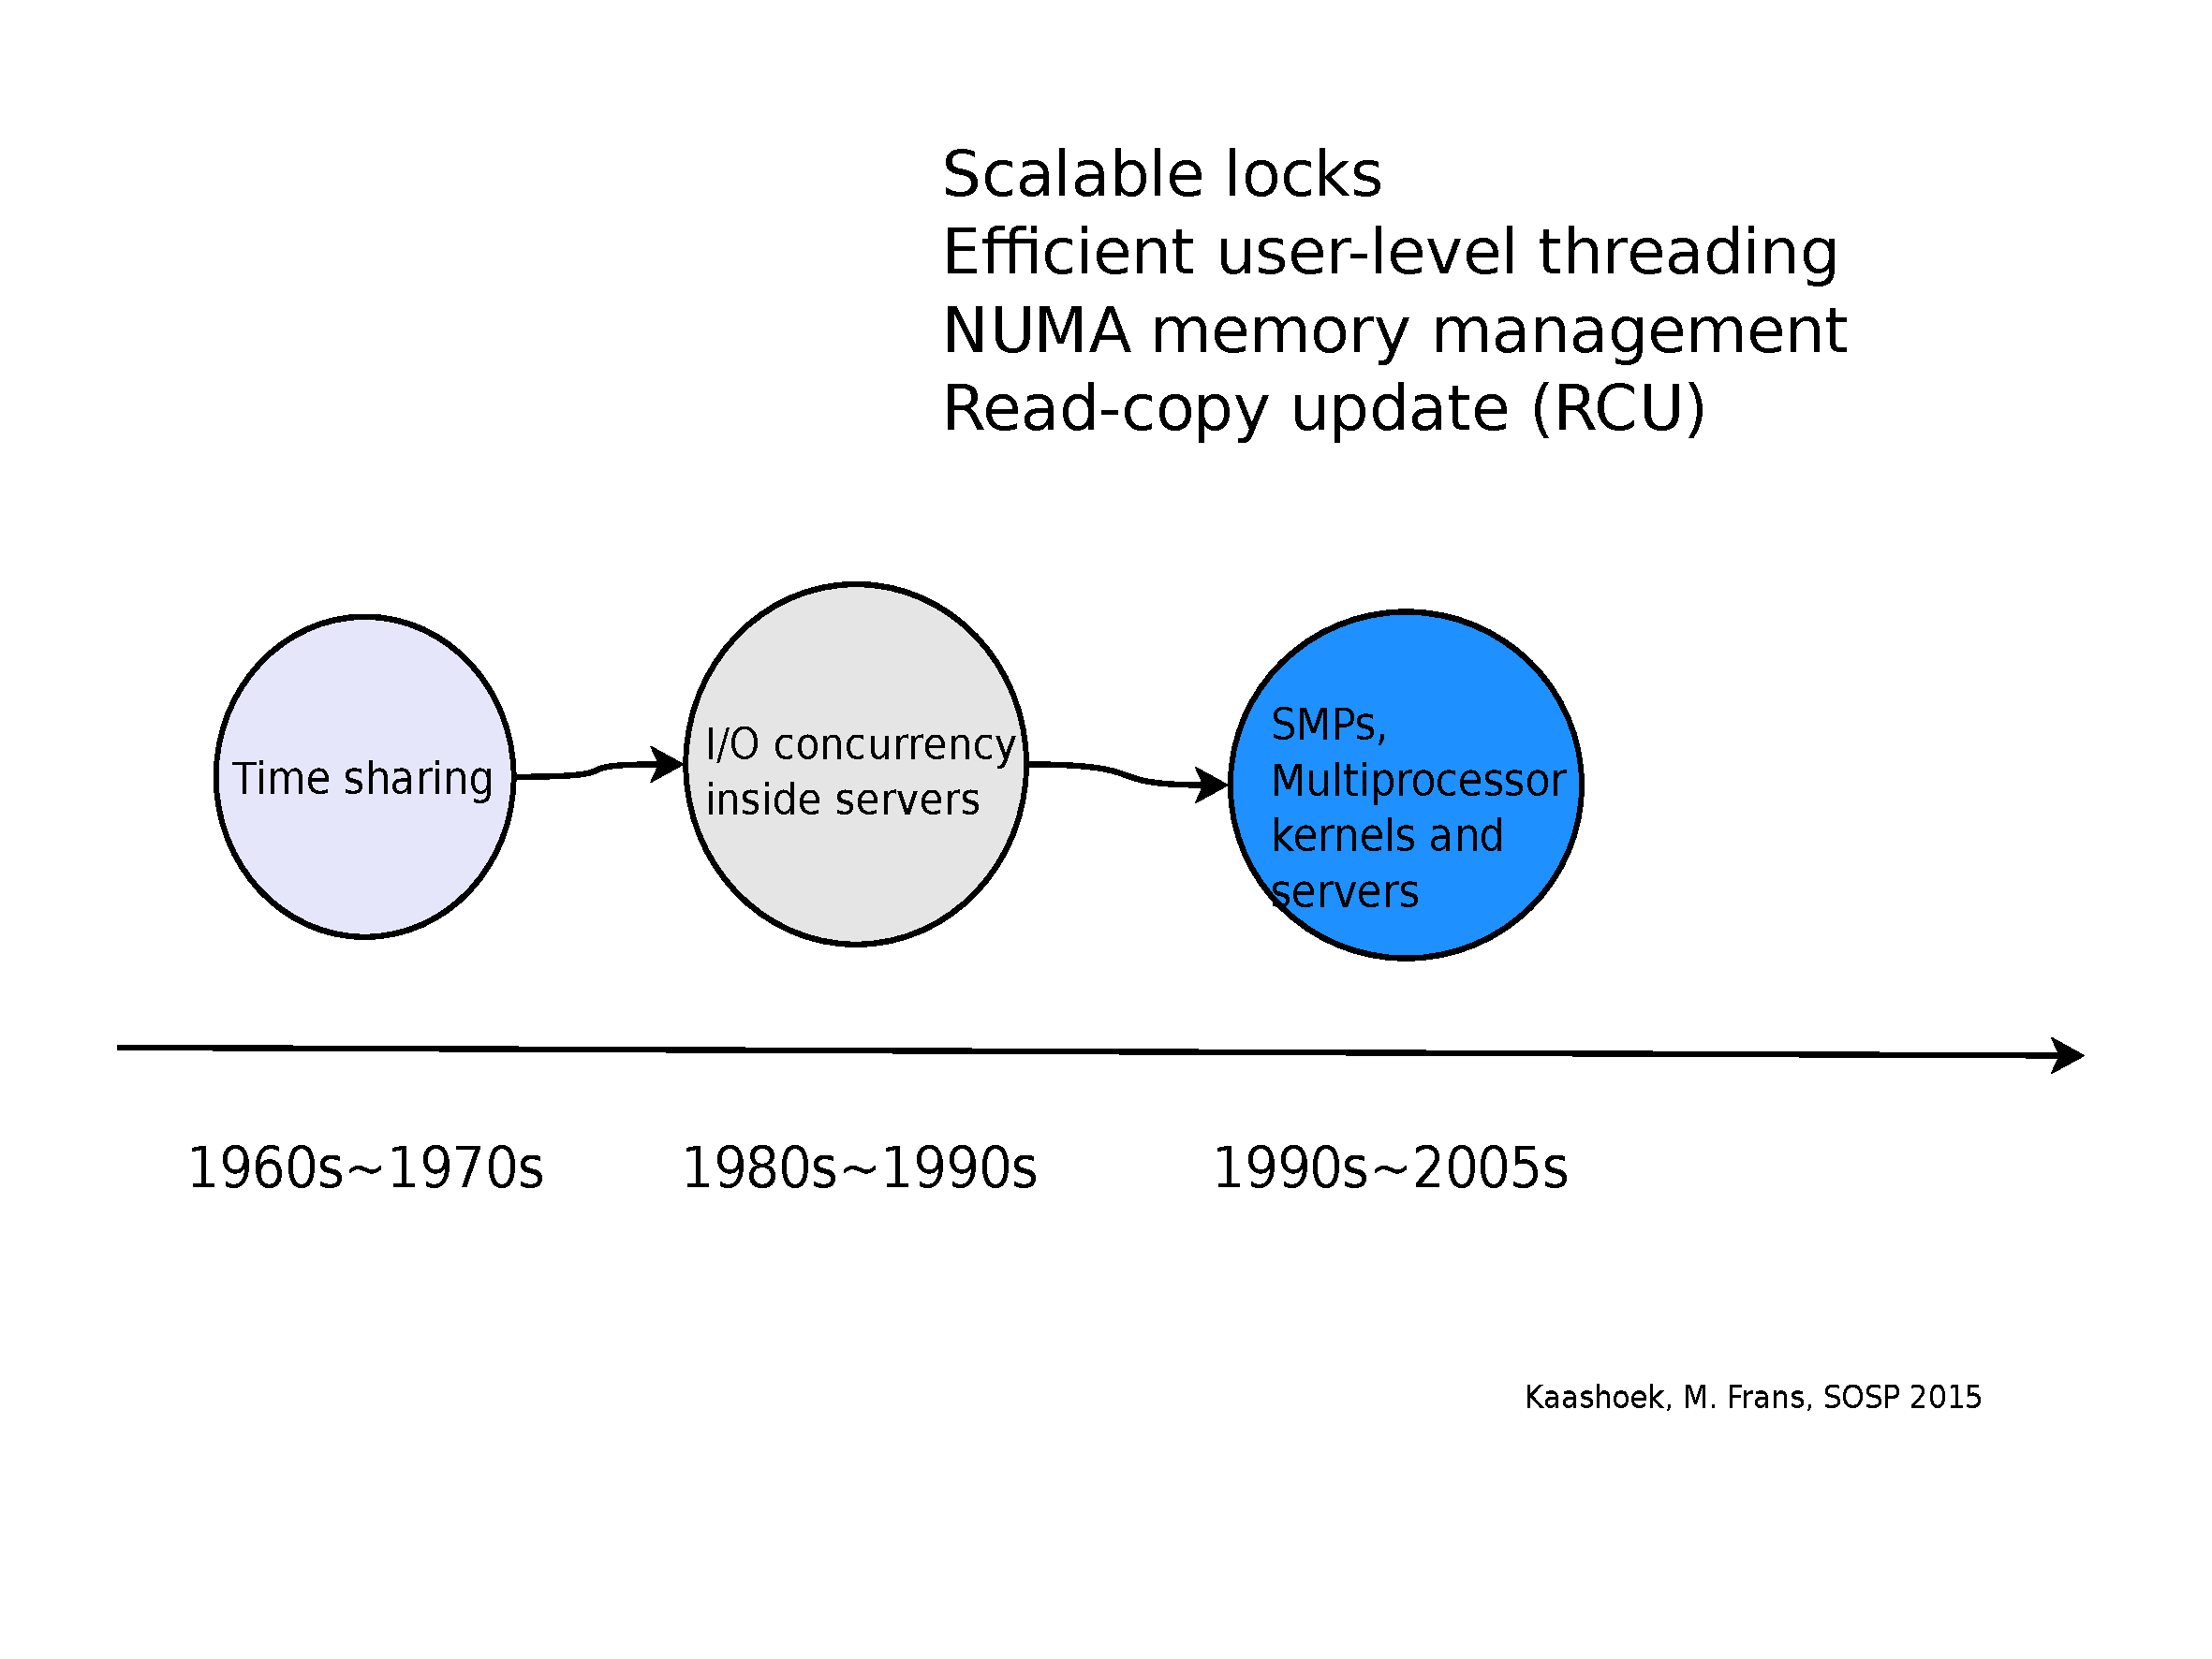
\includegraphics[scale=0.3]{fig/history_old}
\end{center}
\end{frame}


\begin{frame}{40 Years of Microprocessor Trend Data}
\pgfdeclareimage[width=\paperwidth]{cpu_4_1}{.//slides/cpu_4_1}
\begin{textblock}{1}(0,0)
\pgfuseimage<+->{cpu_4_1}
\end{textblock}
\end{frame}


\begin{frame}{Cache-Coherence System}
\begin{center}
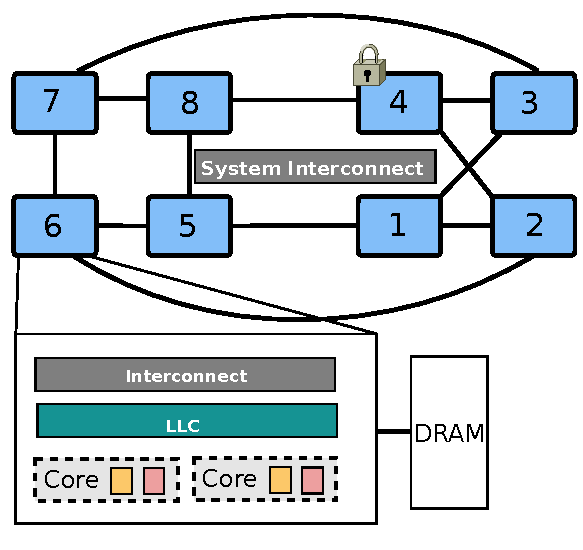
\includegraphics[scale=0.8]{fig/archcache_1}
\end{center}
\end{frame}


\begin{frame}{Cache-Coherence System}
\begin{center}
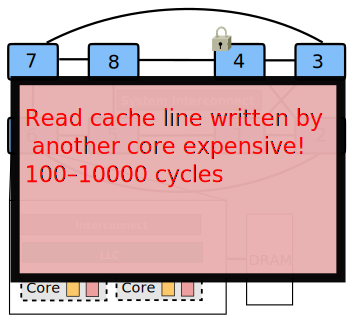
\includegraphics[scale=0.8]{fig/archcache_1_1}
\end{center}
\end{frame}


\begin{frame}{Cache-Coherence System}
\begin{center}
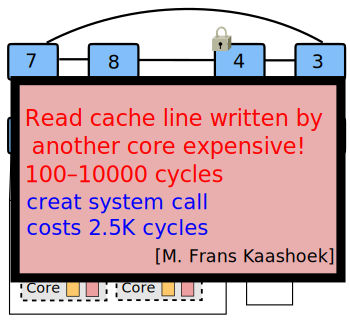
\includegraphics[scale=0.8]{fig/archcache_1_2}
\end{center}
\end{frame}


\begin{frame}{Cache-Coherence System}
\begin{center}
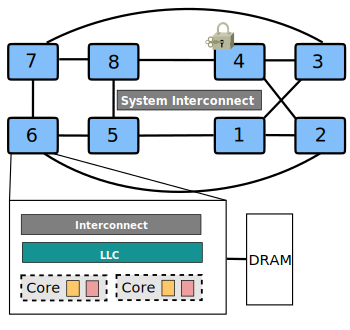
\includegraphics[scale=0.8]{fig/archcache_2}
\end{center}
\end{frame}

\begin{frame}{Cache-Coherence System}
\begin{center}
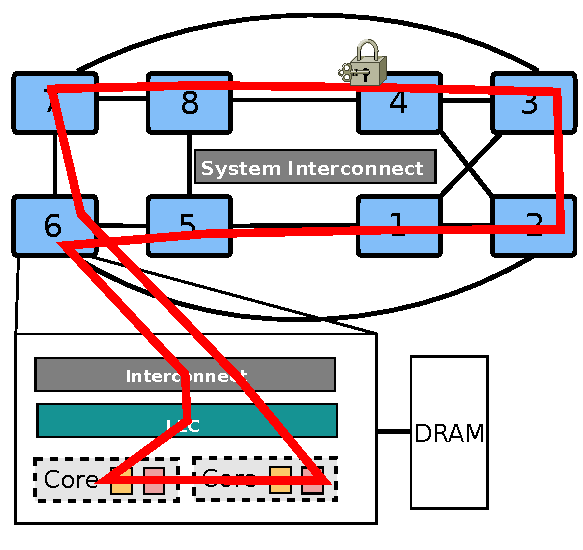
\includegraphics[scale=0.8]{fig/archcache_3}
\end{center}
\end{frame}


\begin{frame}{OS Kernel Scalability History}
\pgfdeclareimage[width=\paperwidth]{history_1}{.//slides/history_1}
\begin{textblock}{1}(0,0)
\pgfuseimage<+->{history_1}
\end{textblock}
\end{frame}



\begin{frame}{OS Kernel Scalability History}
\pgfdeclareimage[width=\paperwidth]{history_2}{.//slides/history_2}
\begin{textblock}{1}(0,0)
\pgfuseimage<+->{history_2}
\end{textblock}
\end{frame}



\begin{frame}{OS Kernel Scalability History}
\pgfdeclareimage[width=\paperwidth]{history_3}{.//slides/history_3}
\begin{textblock}{1}(0,0)
\pgfuseimage<+->{history_3}
\end{textblock}
\end{frame}



\begin{frame}{OS Kernel Scalability History}
\pgfdeclareimage[width=\paperwidth]{history_4}{.//slides/history_4}
\begin{textblock}{1}(0,0)
\pgfuseimage<+->{history_4}
\end{textblock}
\end{frame}



\begin{frame}{OS Kernel Scalability History}
\pgfdeclareimage[width=\paperwidth]{history_5}{.//slides/history_5}
\begin{textblock}{1}(0,0)
\pgfuseimage<+->{history_5}
\end{textblock}
\end{frame}



\begin{frame}{OS Kernel Scalability History}
\pgfdeclareimage[width=\paperwidth]{history_6}{.//slides/history_6}
\begin{textblock}{1}(0,0)
\pgfuseimage<+->{history_6}
\end{textblock}
\end{frame}



\begin{frame}{OS Kernel Scalability History}
\pgfdeclareimage[width=\paperwidth]{history_7}{.//slides/history_7}
\begin{textblock}{1}(0,0)
\pgfuseimage<+->{history_7}
\end{textblock}
\end{frame}



\begin{frame}{Performance Scalability}
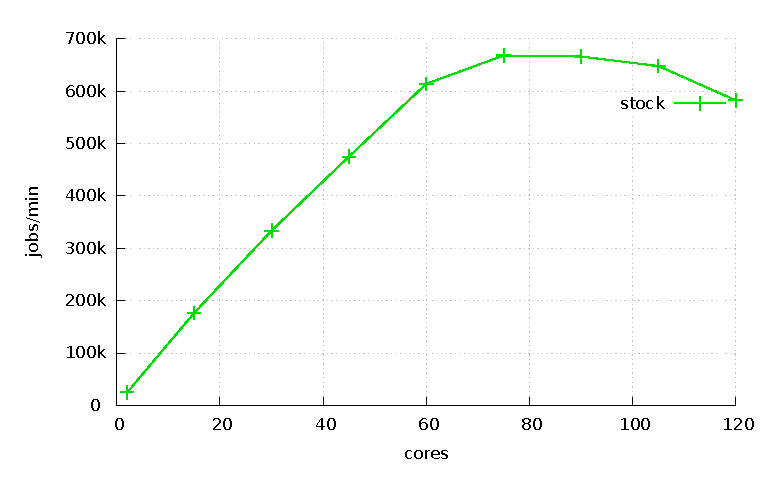
\includegraphics[scale=0.8]{graph/aim7_default}
\end{frame}

\begin{frame}{Performance Scalability}
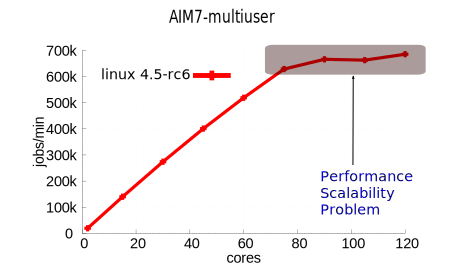
\includegraphics[scale=0.8]{graph/aim7_default_2}
\end{frame}

\begin{frame}{Performance Scalability}
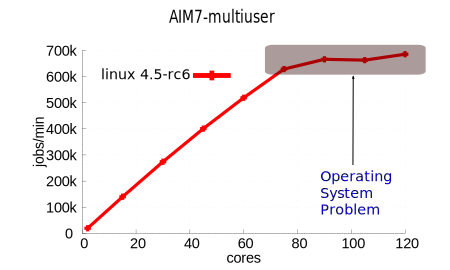
\includegraphics[scale=0.8]{graph/aim7_default_3}
\end{frame}

\begin{frame}{OS Kernel Scalability}
    \begin{itemize}[<+-| alert@+>]
    \item OS kernel scalability is an important part for the whole the system
    parallelism.
    \item If the kernel does not scale, applications will not scale.
    \end{itemize}
\end{frame}


\begin{frame}{Lock Profile on 120 core}
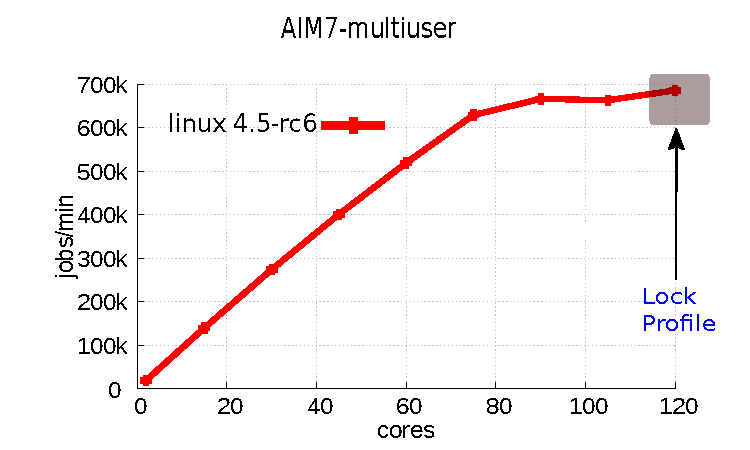
\includegraphics[scale=0.8]{graph/aim7_default_4}
\end{frame}


\begin{frame}{Wait time to acquire the lock}
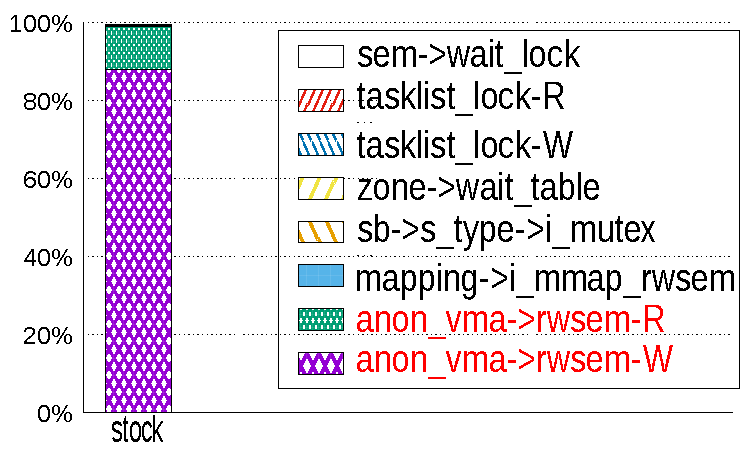
\includegraphics[scale=0.8]{fig/lockstat}
\end{frame}

\begin{frame}{Wait time to acquire the lock}
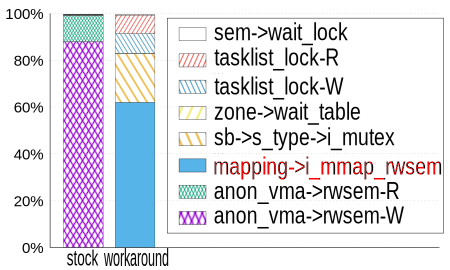
\includegraphics[scale=0.8]{fig/lockstat2}
\end{frame}


\begin{frame}{Update Serialization}
\pgfdeclareimage[width=\paperwidth]{update}{.//slides/update}
\begin{textblock}{1}(0,0)
\pgfuseimage<+->{update}
\end{textblock}
\end{frame}

\begin{frame}{Solution for High Update Rate Data Structure}
    \begin{itemize}[<+-| alert@+>]
    \item Non-blocking Data Structure.
    \begin{itemize}
        \item Harris, Fraser.
    \end{itemize}
    \item Log-based Algorithms. 
    \end{itemize}
\end{frame}


\begin{frame}{Non-blocking Data Structure}
\begin{center}
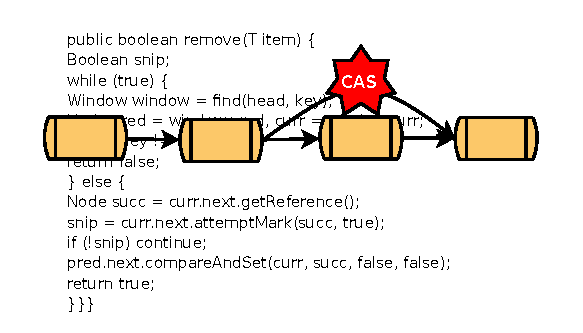
\includegraphics[scale=1.0]{fig/nonblock}
\end{center}
\end{frame}

\begin{frame}{Non-blocking Data Structure}
\begin{center}
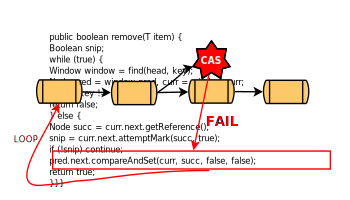
\includegraphics[scale=1.1]{fig/nonblock_fail}
\end{center}
\end{frame}

\begin{frame}{Cache communication bottlenecks}
\begin{center}
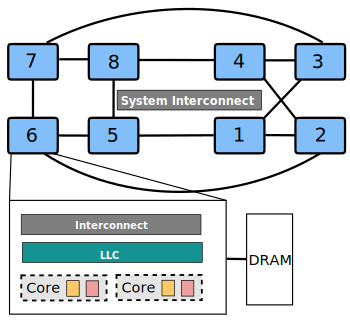
\includegraphics[scale=0.8]{fig/archcache_cas}
\end{center}
\end{frame}

\begin{frame}{Cache communication bottlenecks}
\begin{center}
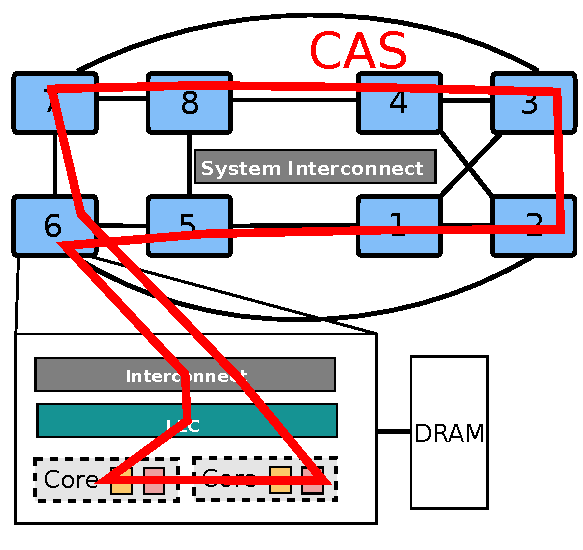
\includegraphics[scale=0.8]{fig/archcache_cas_1}
\end{center}
\end{frame}


\begin{frame}{Log-based Algorithms}
    \begin{itemize}[<+-| alert@+>]
    \item Flat combining(SPAA '10).
    \item OpLog(MIT Ph.D., thesis 2013). 
    \end{itemize}
\end{frame}



\begin{frame}{Log-based Algorithms: OpLog}
\pgfdeclareimage[width=\paperwidth]{oplog_0}{.//slides/oplog_0}
\begin{textblock}{1}(0,0)
\pgfuseimage<+->{oplog_0}
\end{textblock}
\end{frame}


\begin{frame}{Log-based Algorithms: OpLog}
\pgfdeclareimage[width=\paperwidth]{oplog_0_1}{.//slides/oplog_0_1}
\begin{textblock}{1}(0,0)
\pgfuseimage<+->{oplog_0_1}
\end{textblock}
\end{frame}



\begin{frame}{Log-based Algorithms: OpLog}
\pgfdeclareimage[width=\paperwidth]{oplog_1}{.//slides/oplog_1}
\begin{textblock}{1}(0,0)
\pgfuseimage<+->{oplog_1}
\end{textblock}
\end{frame}


\begin{frame}{Log-based Algorithms: OpLog}
\pgfdeclareimage[width=\paperwidth]{oplog_1_1}{.//slides/oplog_1_1}
\begin{textblock}{1}(0,0)
\pgfuseimage<+->{oplog_1_1}
\end{textblock}
\end{frame}


\begin{frame}{Log-based Algorithms: OpLog}
\pgfdeclareimage[width=\paperwidth]{oplog_2}{.//slides/oplog_2}
\begin{textblock}{1}(0,0)
\pgfuseimage<+->{oplog_2}
\end{textblock}
\end{frame}

\begin{frame}{Log-based Algorithms: OpLog}
\pgfdeclareimage[width=\paperwidth]{oplog_2_1}{.//slides/oplog_2_1}
\begin{textblock}{1}(0,0)
\pgfuseimage<+->{oplog_2_1}
\end{textblock}
\end{frame}



\begin{frame}{Log-based Algorithms: OpLog}
\pgfdeclareimage[width=\paperwidth]{oplog}{.//slides/oplog_3}
\begin{textblock}{1}(0,0)
\pgfuseimage<+->{oplog}
\end{textblock}
\end{frame}


\begin{frame}{Time-stamp counters}
\pgfdeclareimage[width=\paperwidth]{oplog_max}{.//slides/oplog_max}
\begin{textblock}{1}(0,0)
\pgfuseimage<+->{oplog_max}
\end{textblock}
\end{frame}

\begin{frame}{Simple Solution?}
\end{frame}

\begin{frame}{Simple Solution}
    \begin{itemize}[<+-| alert@+>]
    \item A Lightweight Log-based Deferred Update(LDU).
    \end{itemize}
\end{frame}


\begin{frame}{Contributions}
    \begin{itemize}[<+-| alert@+>]
	\item Removing time-stamp counters.
	\item Applying the LDU to two reverse mapping(anonymous, file).
	\item Improved throughput and execution time from 1.5x through 2.7x
	on 120 core.
	\end{itemize}
\end{frame}


\begin{frame}{Outline}
	\begin{itemize}
	\item Design
	\begin{itemize}
	\item Approach
	\item Example 
	\end{itemize}
	\item Applying the Linux kernel
	\item Implementation
	\item Evaluation
	\end{itemize}
\end{frame}



\begin{frame}{Why the OpLog needs the time-stamp counter?}
\textit{``A process logs an insert operation to the per-core memory, then
it migrates to another core, and it logs a remove operation, which must
eventually execute after the insert operation''}, OpLog.
\end{frame}



\begin{frame}{Log Example}
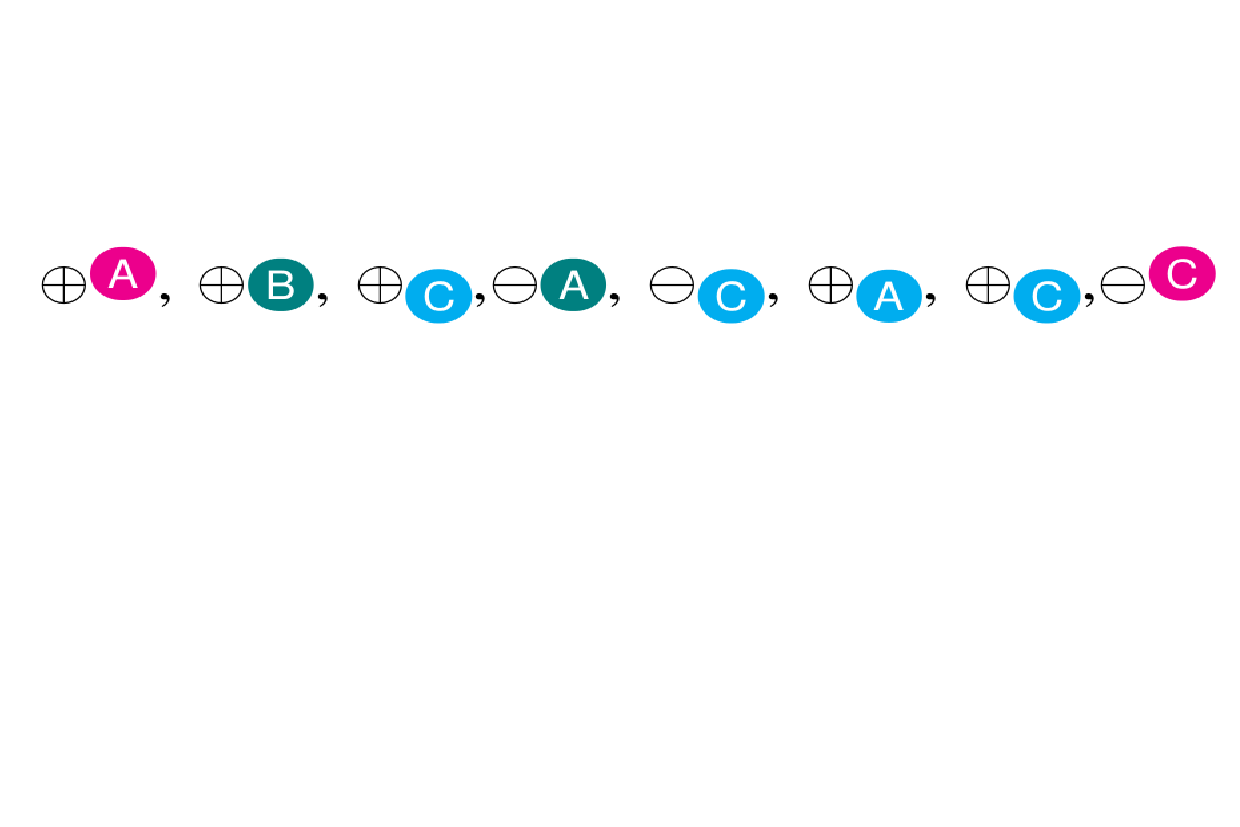
\includegraphics[scale=0.5]{fig/example_1}
\end{frame}


\begin{frame}{Cancelable - Log}
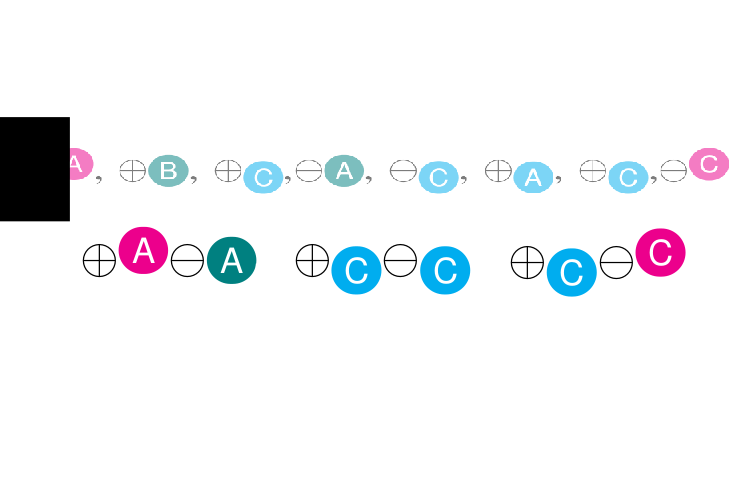
\includegraphics[scale=0.5]{fig/example_2}
\end{frame}


\begin{frame}{Remain Log}
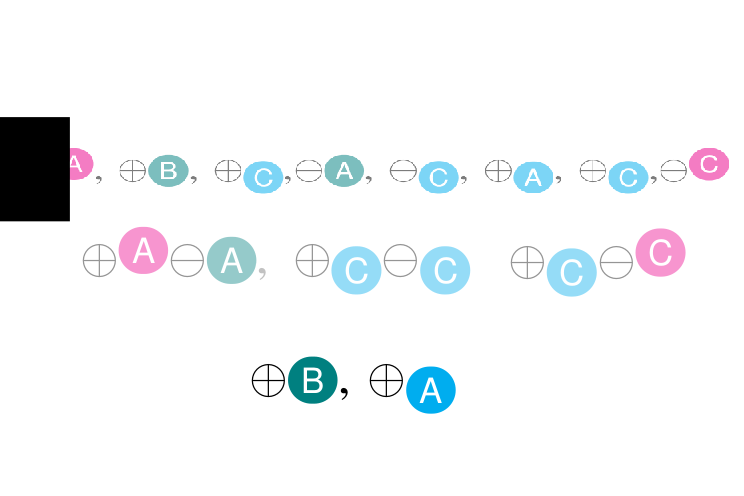
\includegraphics[scale=0.5]{fig/example_3}
\end{frame}


\begin{frame}{Update-side removing}
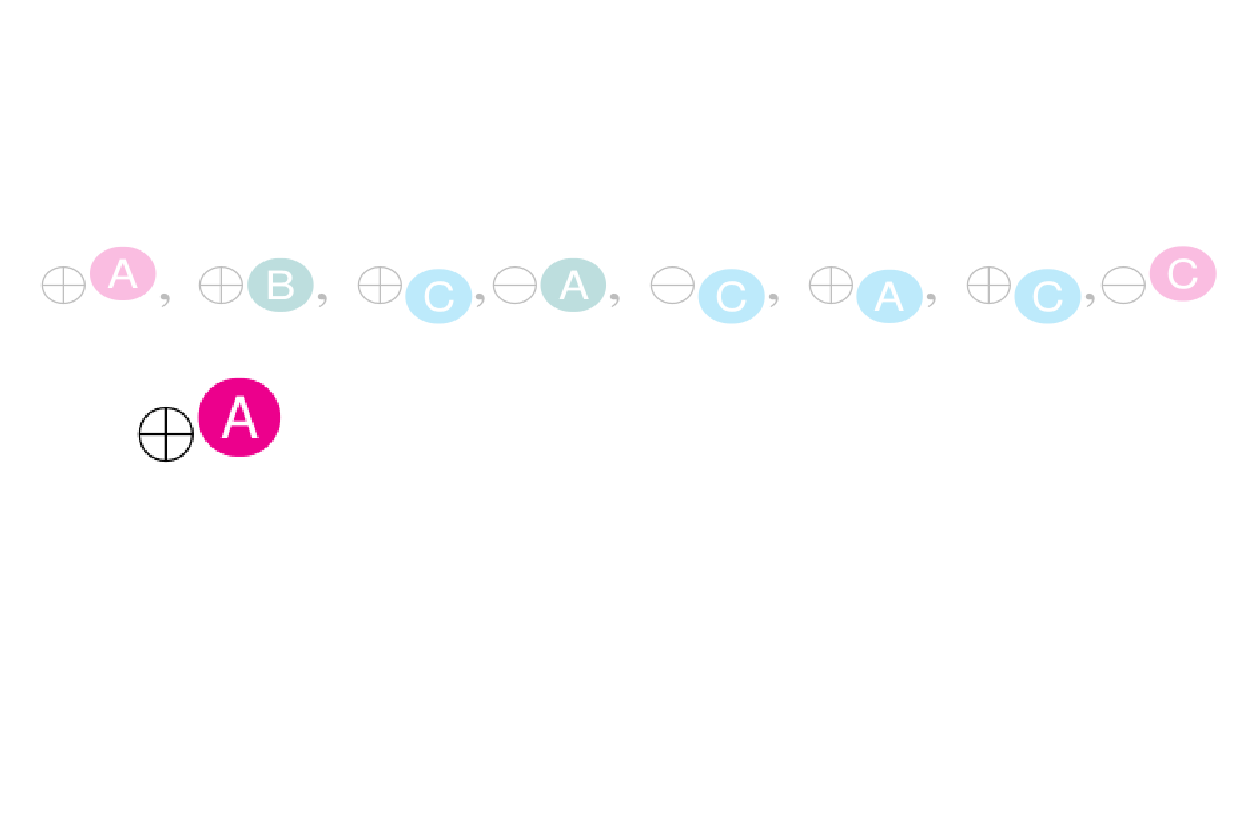
\includegraphics[scale=0.5]{fig/update_remove_0}
\end{frame}

\begin{frame}{Update-side removing}
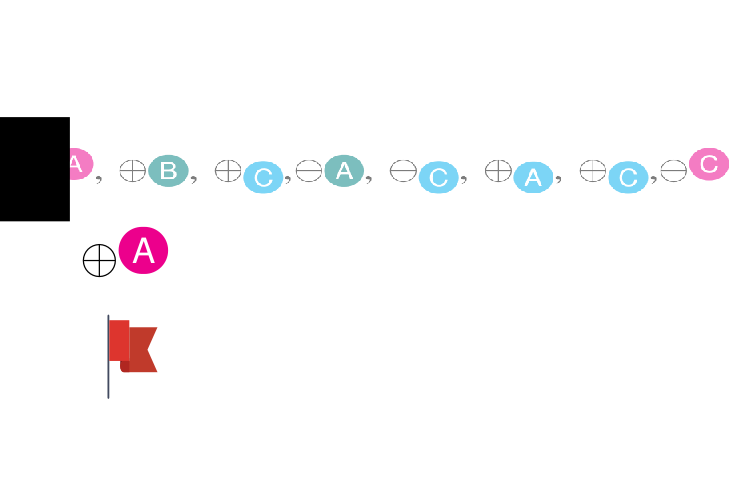
\includegraphics[scale=0.5]{fig/update_remove_1}
\end{frame}

\begin{frame}{Update-side removing}
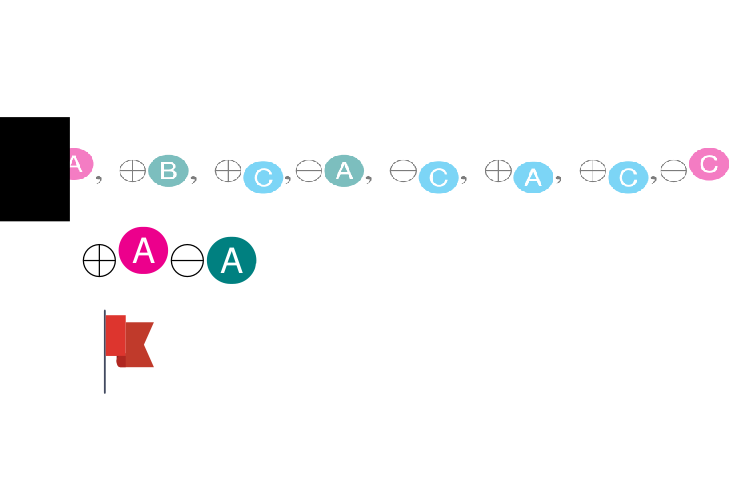
\includegraphics[scale=0.5]{fig/update_remove_2}
\end{frame}


\begin{frame}{Update-side removing}
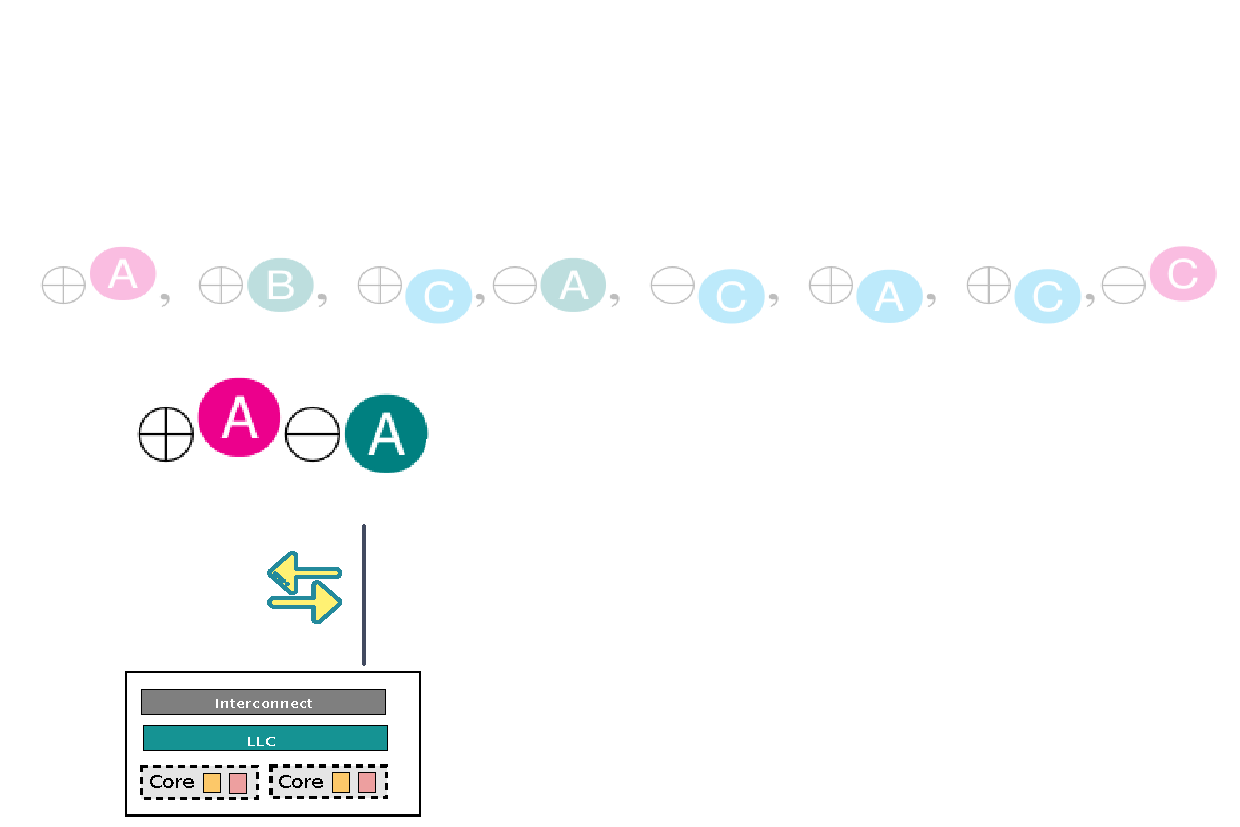
\includegraphics[scale=0.5]{fig/update_remove_2-1}
\end{frame}


\begin{frame}{Update-side removing}
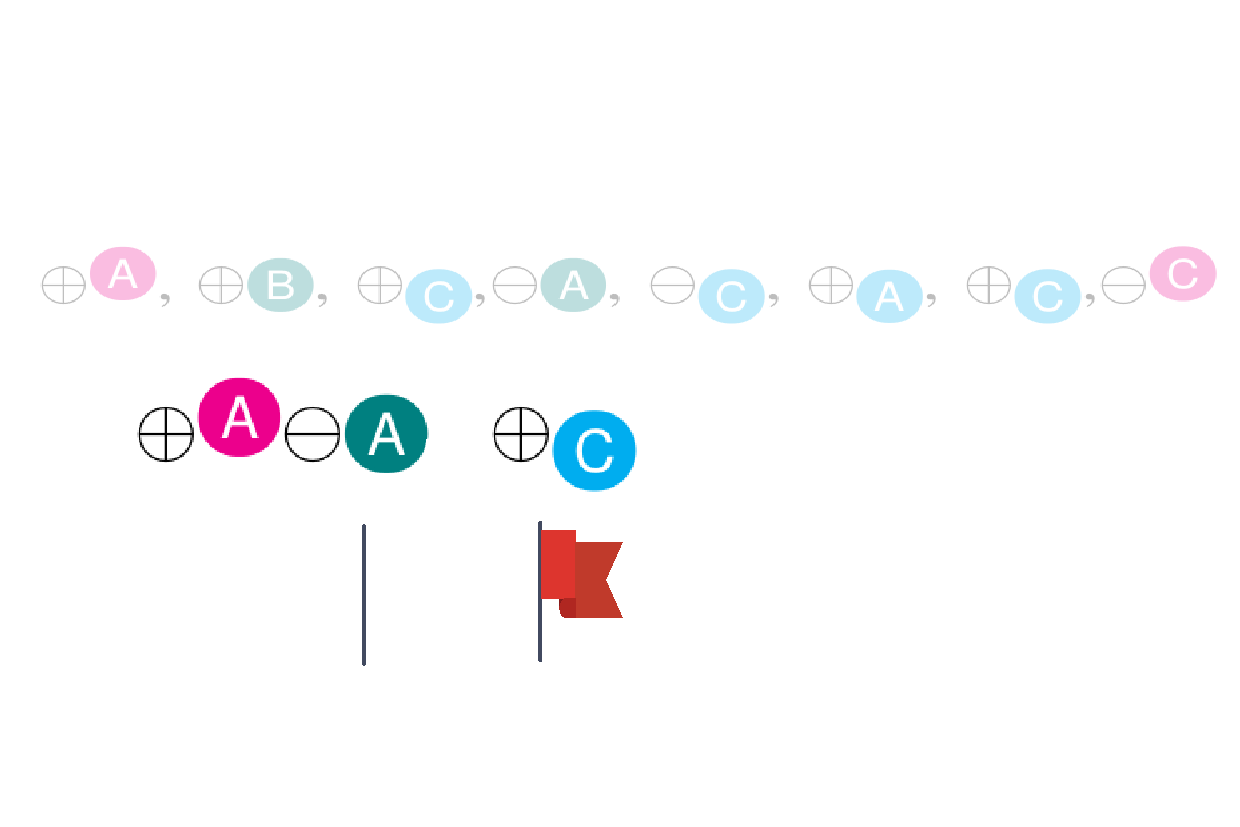
\includegraphics[scale=0.5]{fig/update_remove_3}
\end{frame}

\begin{frame}{Update-side removing}
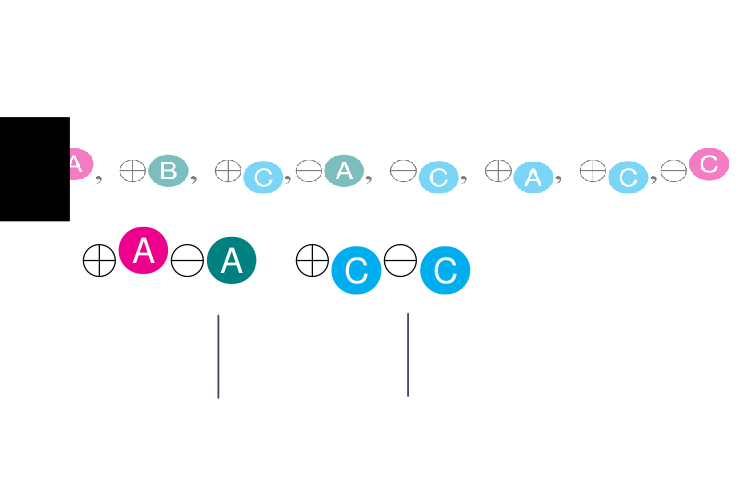
\includegraphics[scale=0.5]{fig/update_remove_4}
\end{frame}


\begin{frame}{Reusing garbage }
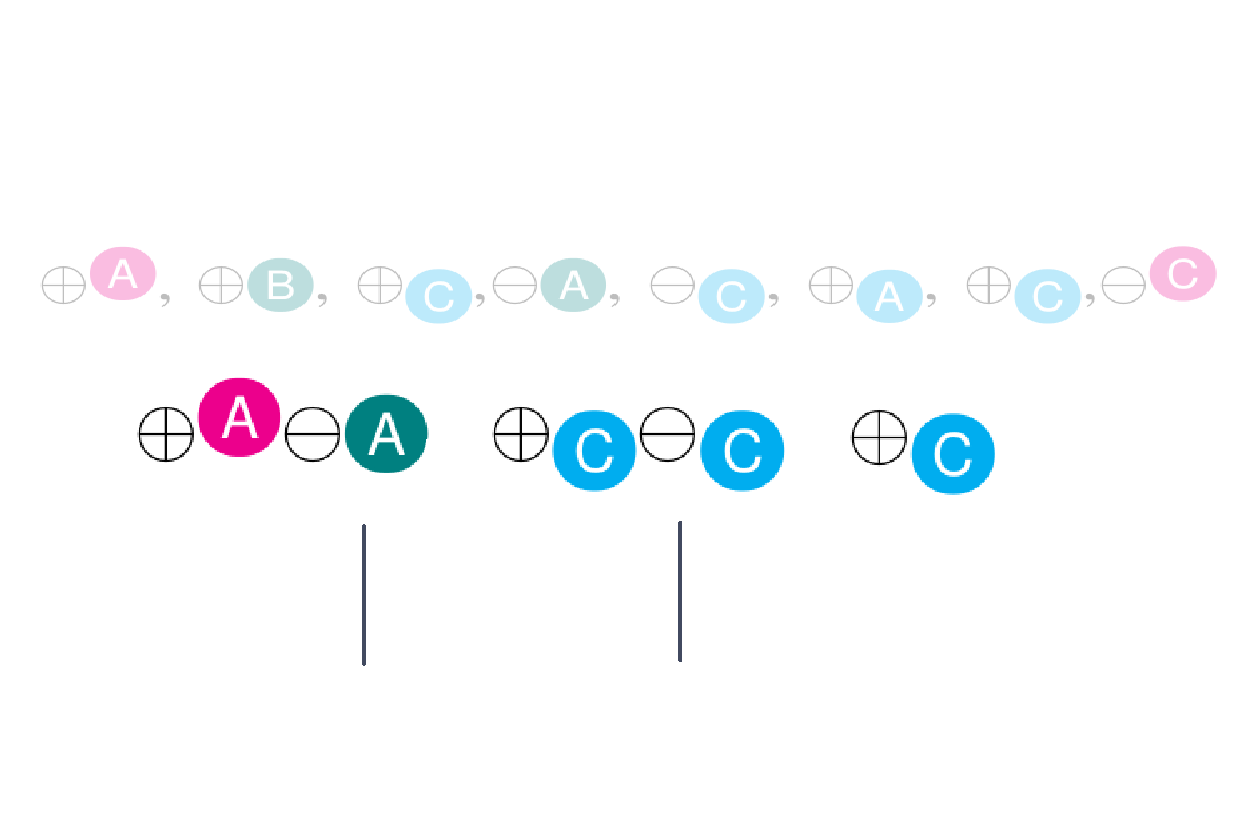
\includegraphics[scale=0.5]{fig/reusing_garbage_1}
\end{frame}

\begin{frame}{Reusing garbage }
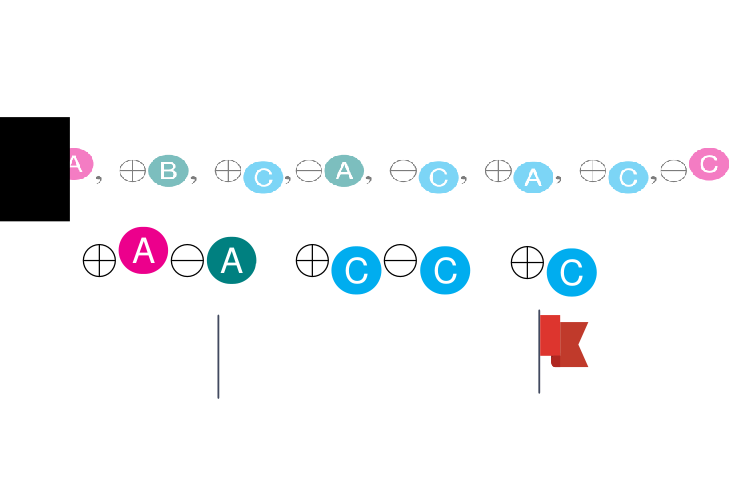
\includegraphics[scale=0.5]{fig/reusing_garbage_2}
\end{frame}

\begin{frame}{Additional approach}
	\begin{itemize}
	\item Periodically applies the operation logs.
	\begin{itemize}
	\item To reduce memory usage and to keep the log from growing without
	end.
	\item Similar with the method of previous OpLog’s batching
	updates and flat combining(FC)’s combiner thread.
	\end{itemize}
	\item Use non-blocking queue.
	\begin{itemize}
	  \item Regardless of the per-core queue or the global
	  queue.
	  \item Multiple producers and single consumer based non-blocking queue
	  thereby reducing the CAS operations.
	\end{itemize}
	\end{itemize}
\end{frame}


\begin{frame}{Example}
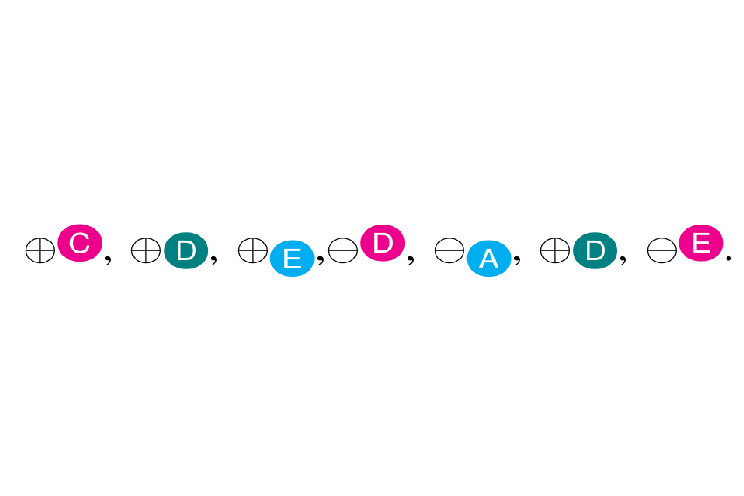
\includegraphics[scale=0.5]{fig/example}
\end{frame}


\begin{frame}{Example}
\pgfdeclareimage[width=\paperwidth]{ldu_1}{.//slides/ldu_1}
\begin{textblock}{1}(0,0)
\pgfuseimage<+->{ldu_1}
\end{textblock}
\end{frame}

\begin{frame}{Example}
\pgfdeclareimage[width=\paperwidth]{ldu_2}{.//slides/ldu_2}
\begin{textblock}{1}(0,0)
\pgfuseimage<+->{ldu_2}
\end{textblock}
\end{frame}

\begin{frame}{Example}
\pgfdeclareimage[width=\paperwidth]{ldu_3}{.//slides/ldu_3}
\begin{textblock}{1}(0,0)
\pgfuseimage<+->{ldu_3}
\end{textblock}
\end{frame}


\begin{frame}{Example}
\pgfdeclareimage[width=\paperwidth]{ldu_4}{.//slides/ldu_4}
\begin{textblock}{1}(0,0)
\pgfuseimage<+->{ldu_4}
\end{textblock}
\end{frame}


\begin{frame}{Example}
\pgfdeclareimage[width=\paperwidth]{ldu_5}{.//slides/ldu_5}
\begin{textblock}{1}(0,0)
\pgfuseimage<+->{ldu_5}
\end{textblock}
\end{frame}


\begin{frame}{Example}
\pgfdeclareimage[width=\paperwidth]{ldu_6}{.//slides/ldu_6}
\begin{textblock}{1}(0,0)
\pgfuseimage<+->{ldu_6}
\end{textblock}
\end{frame}


\begin{frame}{Example}
\pgfdeclareimage[width=\paperwidth]{ldu_7}{.//slides/ldu_7}
\begin{textblock}{1}(0,0)
\pgfuseimage<+->{ldu_7}
\end{textblock}
\end{frame}


\begin{frame}{Example}
\pgfdeclareimage[width=\paperwidth]{ldu_8}{.//slides/ldu_8}
\begin{textblock}{1}(0,0)
\pgfuseimage<+->{ldu_8}
\end{textblock}
\end{frame}


\begin{frame}{Example}
\pgfdeclareimage[width=\paperwidth]{ldu_9}{.//slides/ldu_9}
\begin{textblock}{1}(0,0)
\pgfuseimage<+->{ldu_9}
\end{textblock}
\end{frame}

\begin{frame}{Example}
\pgfdeclareimage[width=\paperwidth]{ldu_10}{.//slides/ldu_10}
\begin{textblock}{1}(0,0)
\pgfuseimage<+->{ldu_10}
\end{textblock}
\end{frame}


\begin{frame}{Applying the Linux kernel}
    \begin{itemize}[<+-| alert@+>]
    \item The Linux reverse page mapping(rmap).
    \item Kernel memory management mechanism.
    \item Consists of anonymous rmap and file rmap.
    \item Update-heavy data structure.
    \end{itemize}
\end{frame}

\begin{frame}{Anonymous reverse mapping}
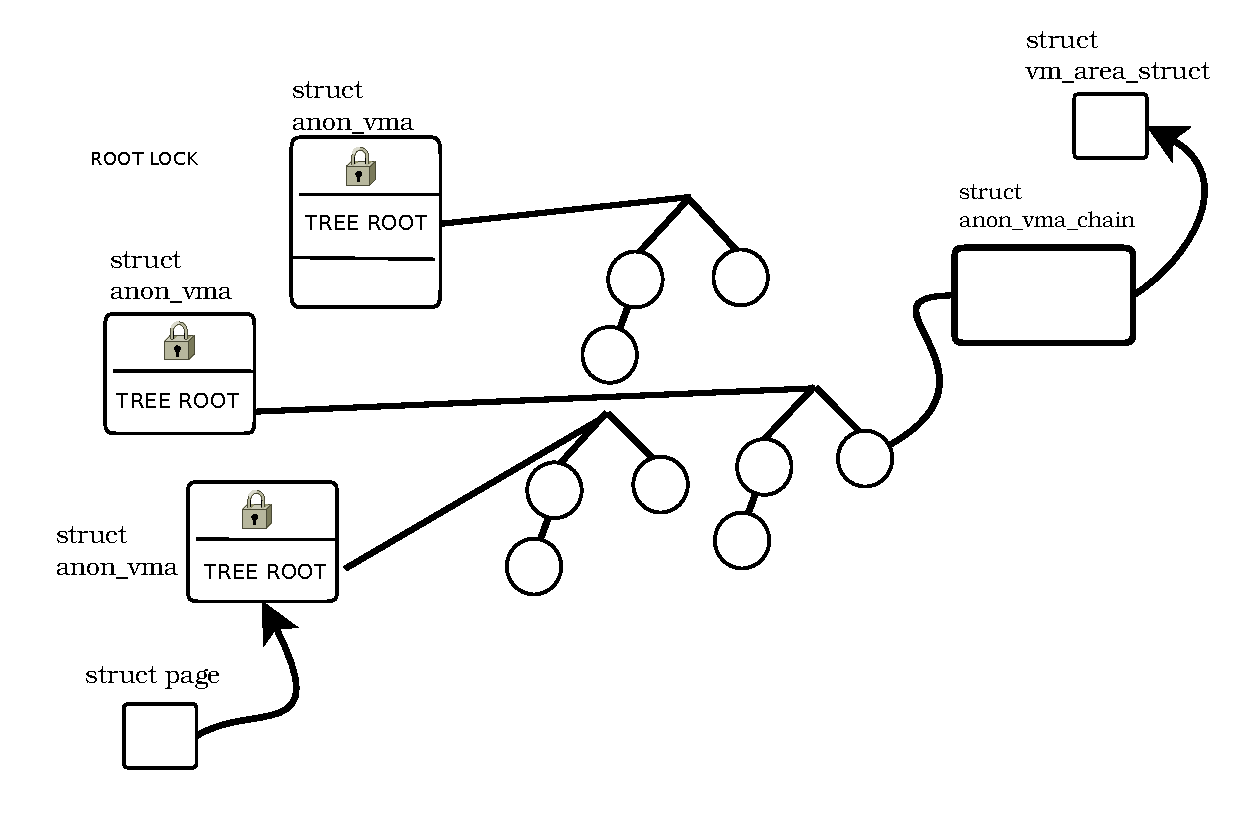
\includegraphics[scale=0.5]{fig/anon_vma_default_0}
\end{frame}


\begin{frame}{Anonymous reverse mapping}
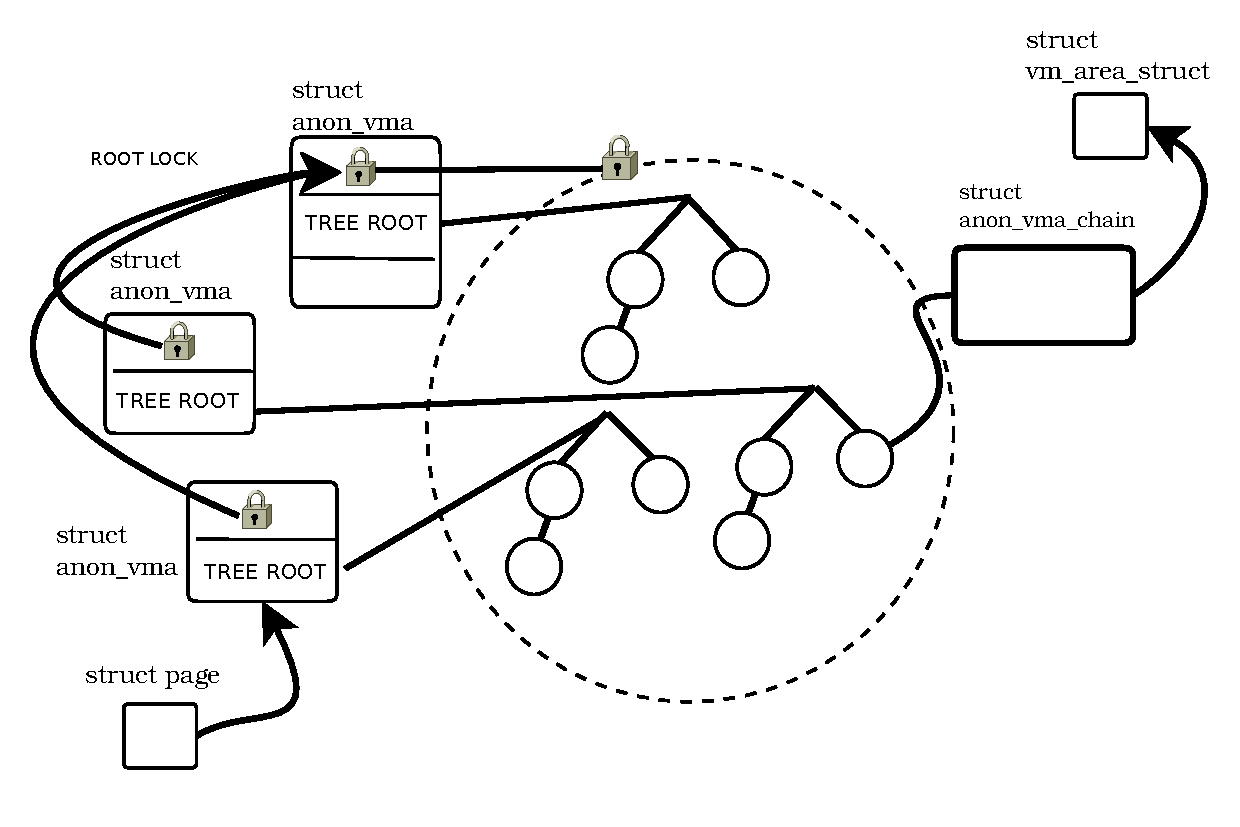
\includegraphics[scale=0.5]{fig/anon_vma_default}
\end{frame}


\begin{frame}{Anonymous reverse mapping}
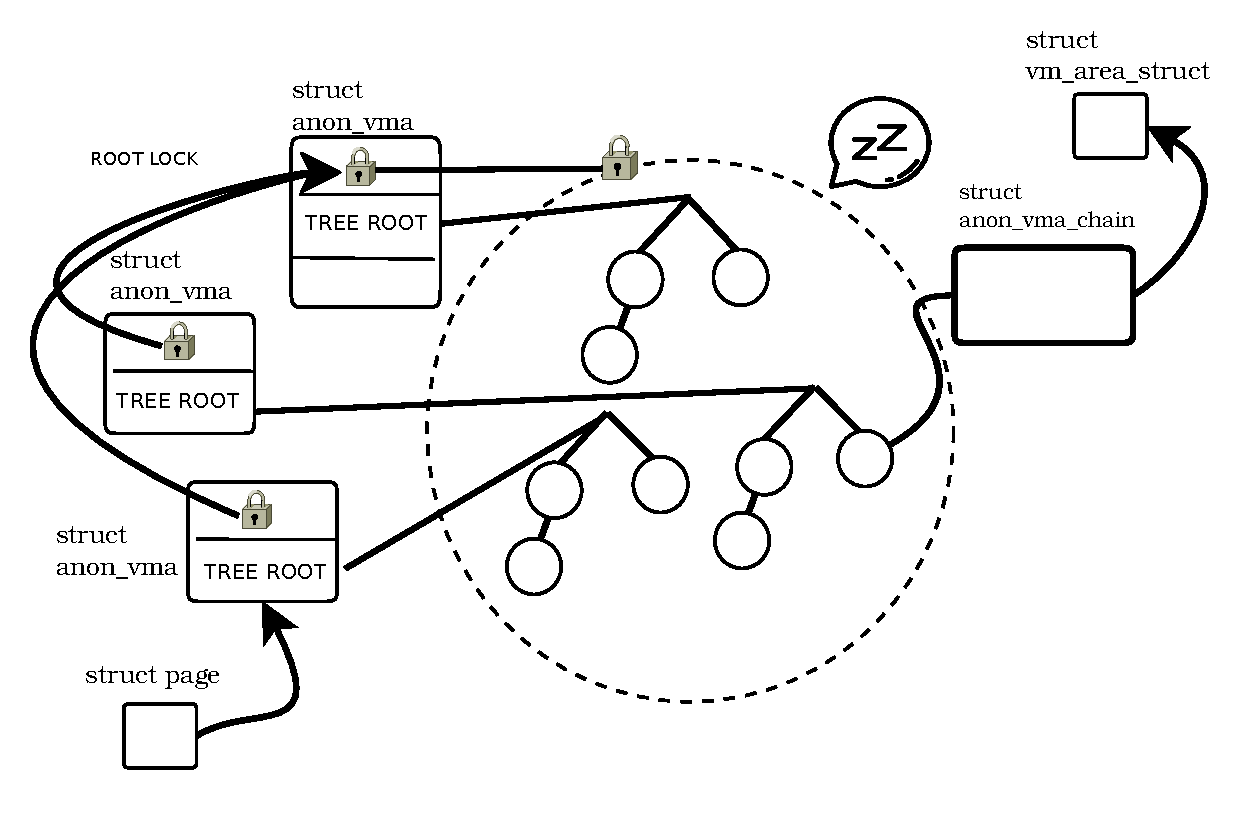
\includegraphics[scale=0.5]{fig/anon_vma_default_1}
\end{frame}


\begin{frame}{Anonymous reverse mapping}
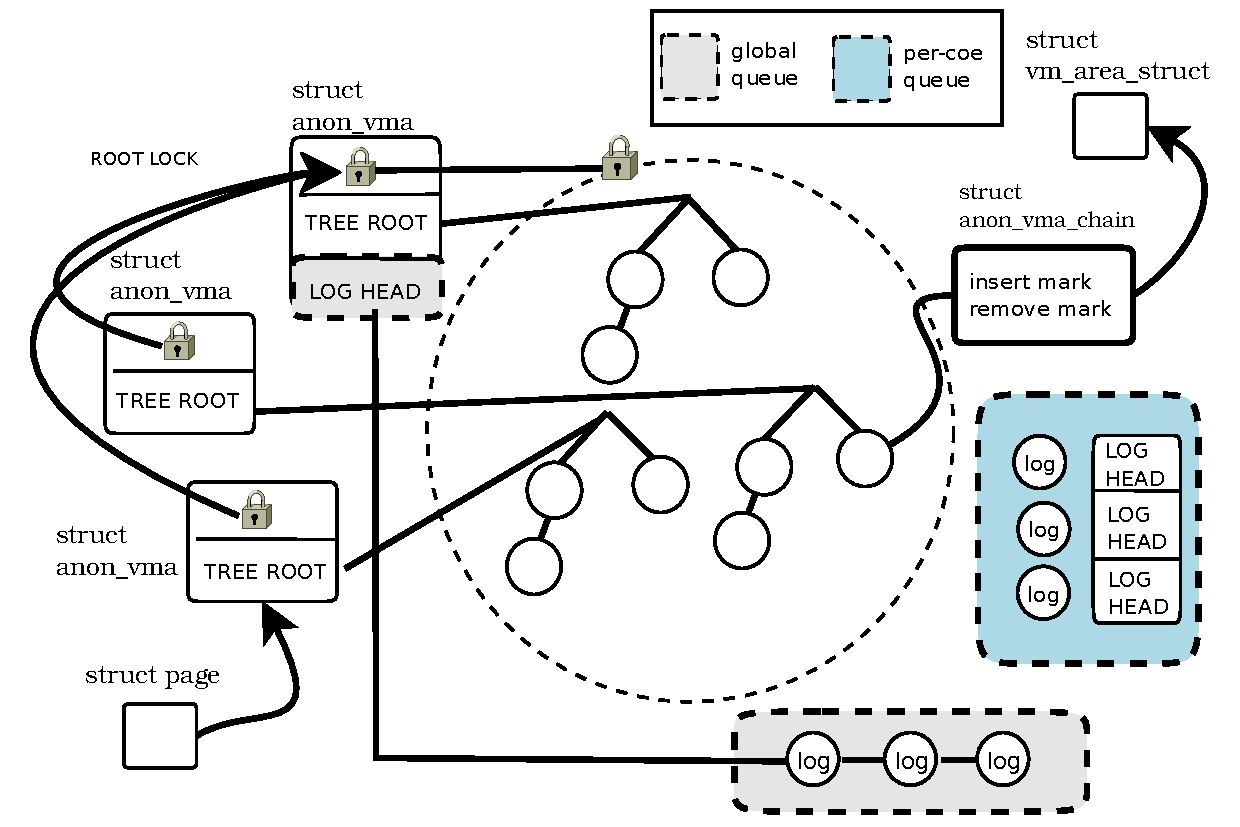
\includegraphics[scale=0.5]{fig/anon_vma}
\end{frame}


\begin{frame}{File mapping}
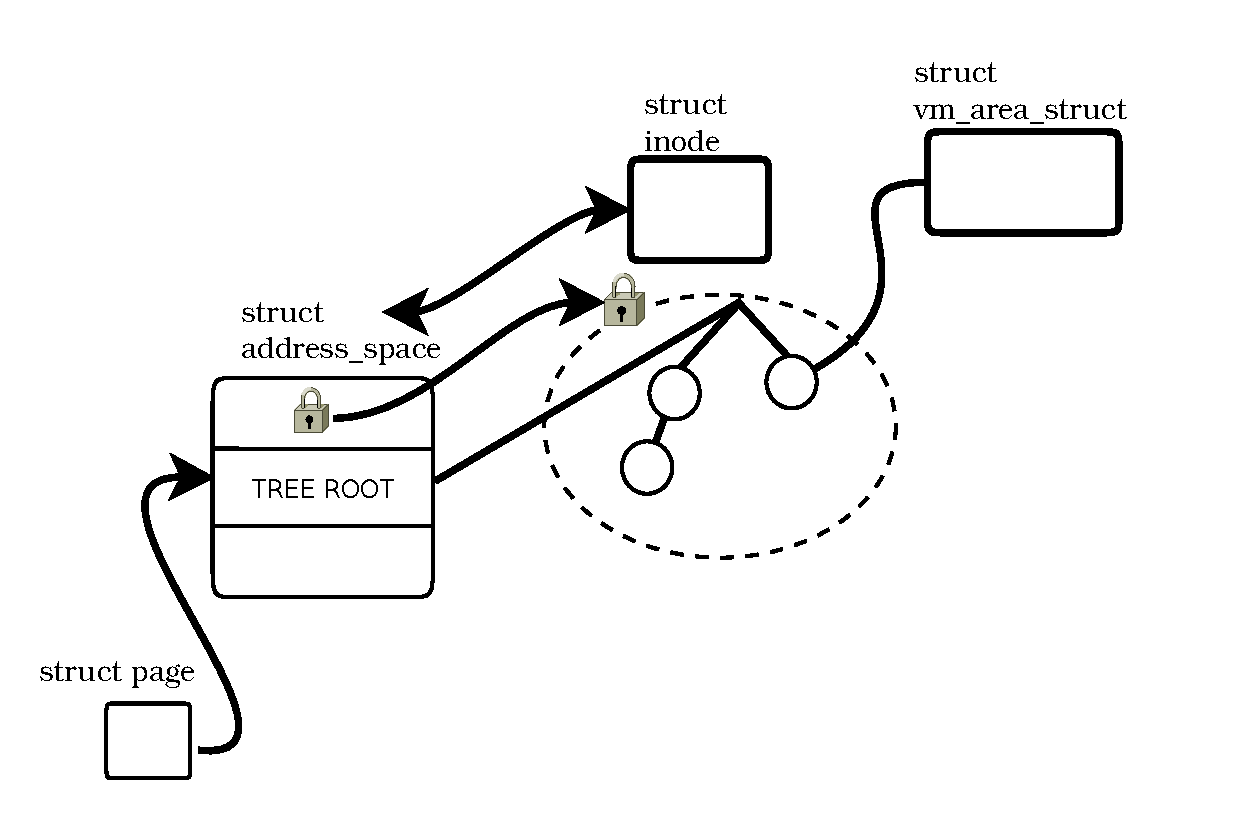
\includegraphics[scale=0.5]{fig/file_rmap_default}
\end{frame}


\begin{frame}{File mapping}
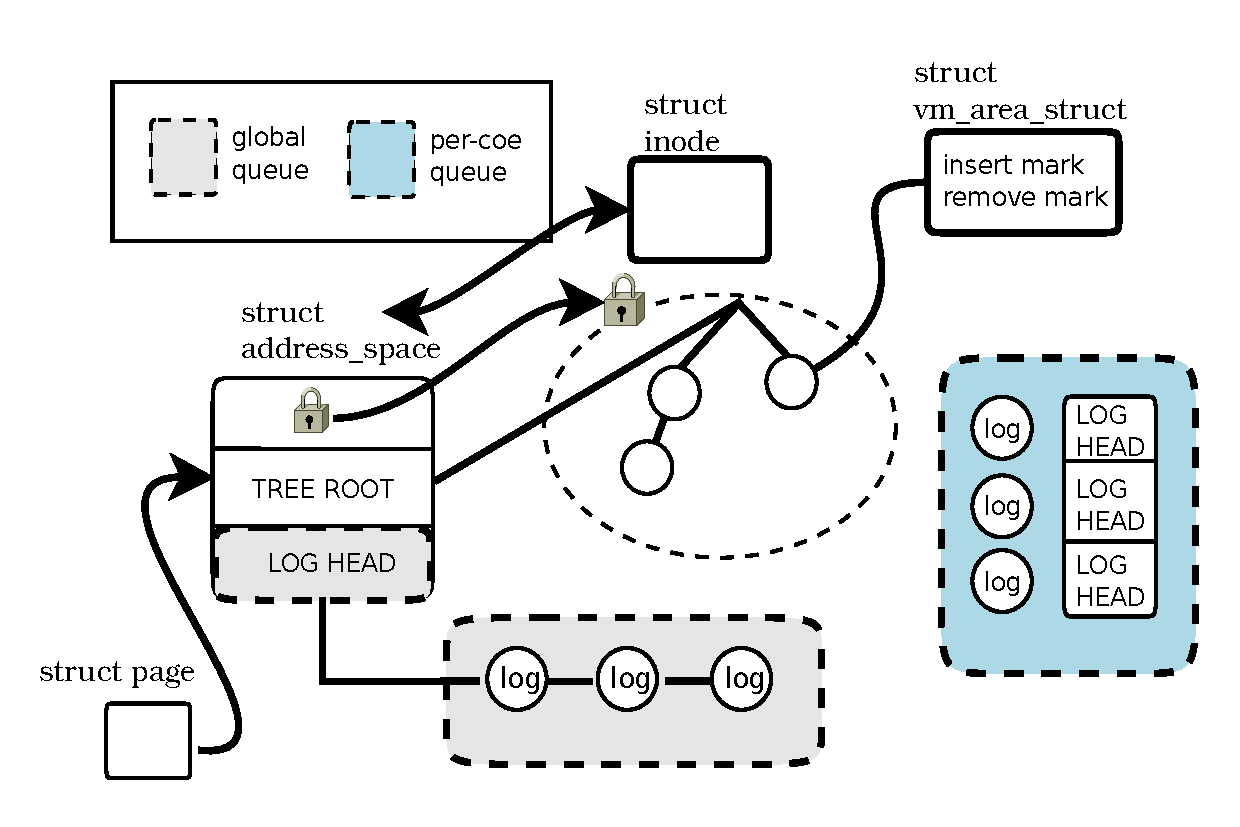
\includegraphics[scale=0.5]{fig/file_rmap}
\end{frame}



\begin{frame}{Evaluation}
    \begin{itemize}[<+-| alert@+>]
    \item We used four different experiment settings.
    \item 1. stock Linux
    \item 2. LDU + global queue
    \item 3. LDU + per-core queue
    \item 4. Harris linked list
    \end{itemize}
\end{frame}

\begin{frame}{Non-blocking algorithm - Harris linked list}
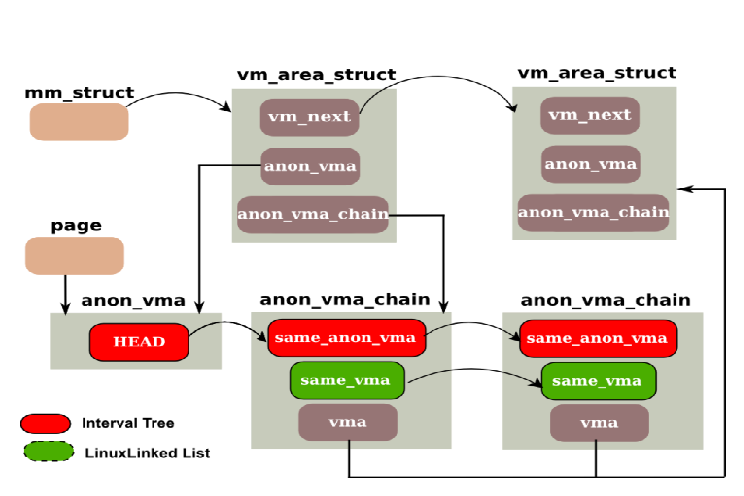
\includegraphics[scale=0.5]{fig/lockfree}
\end{frame}


\begin{frame}{Non-blocking algorithm - Harris linked list}
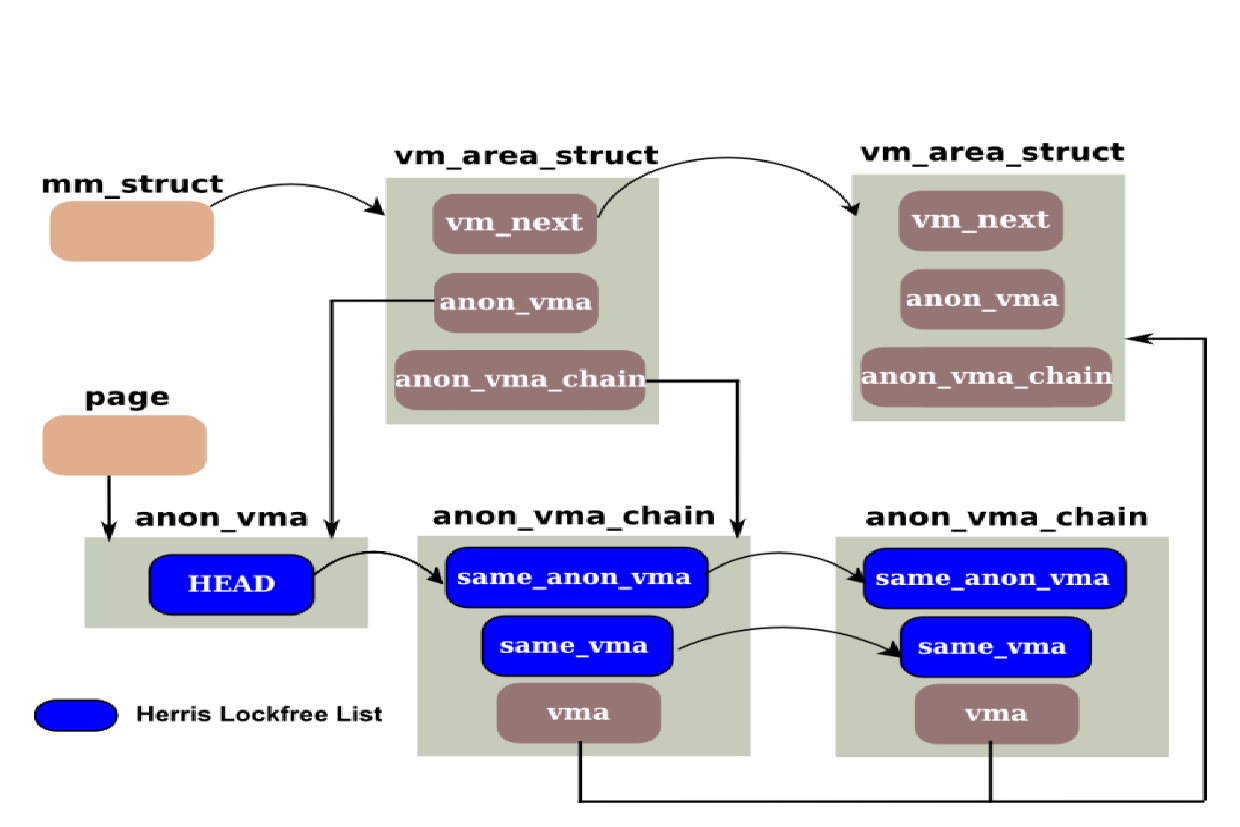
\includegraphics[scale=0.5]{fig/lockfree_2}
\end{frame}

\begin{frame}{Evaluation : Hardware}
\begin{center}
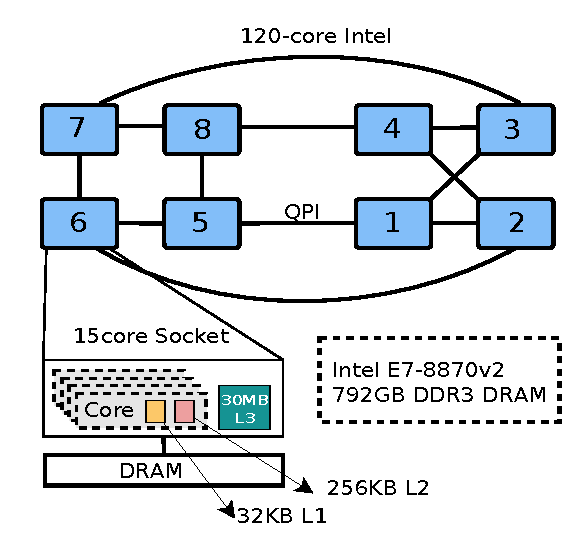
\includegraphics[scale=0.8]{fig/xeon}
\end{center}
\end{frame}


\begin{frame}{AIM7}
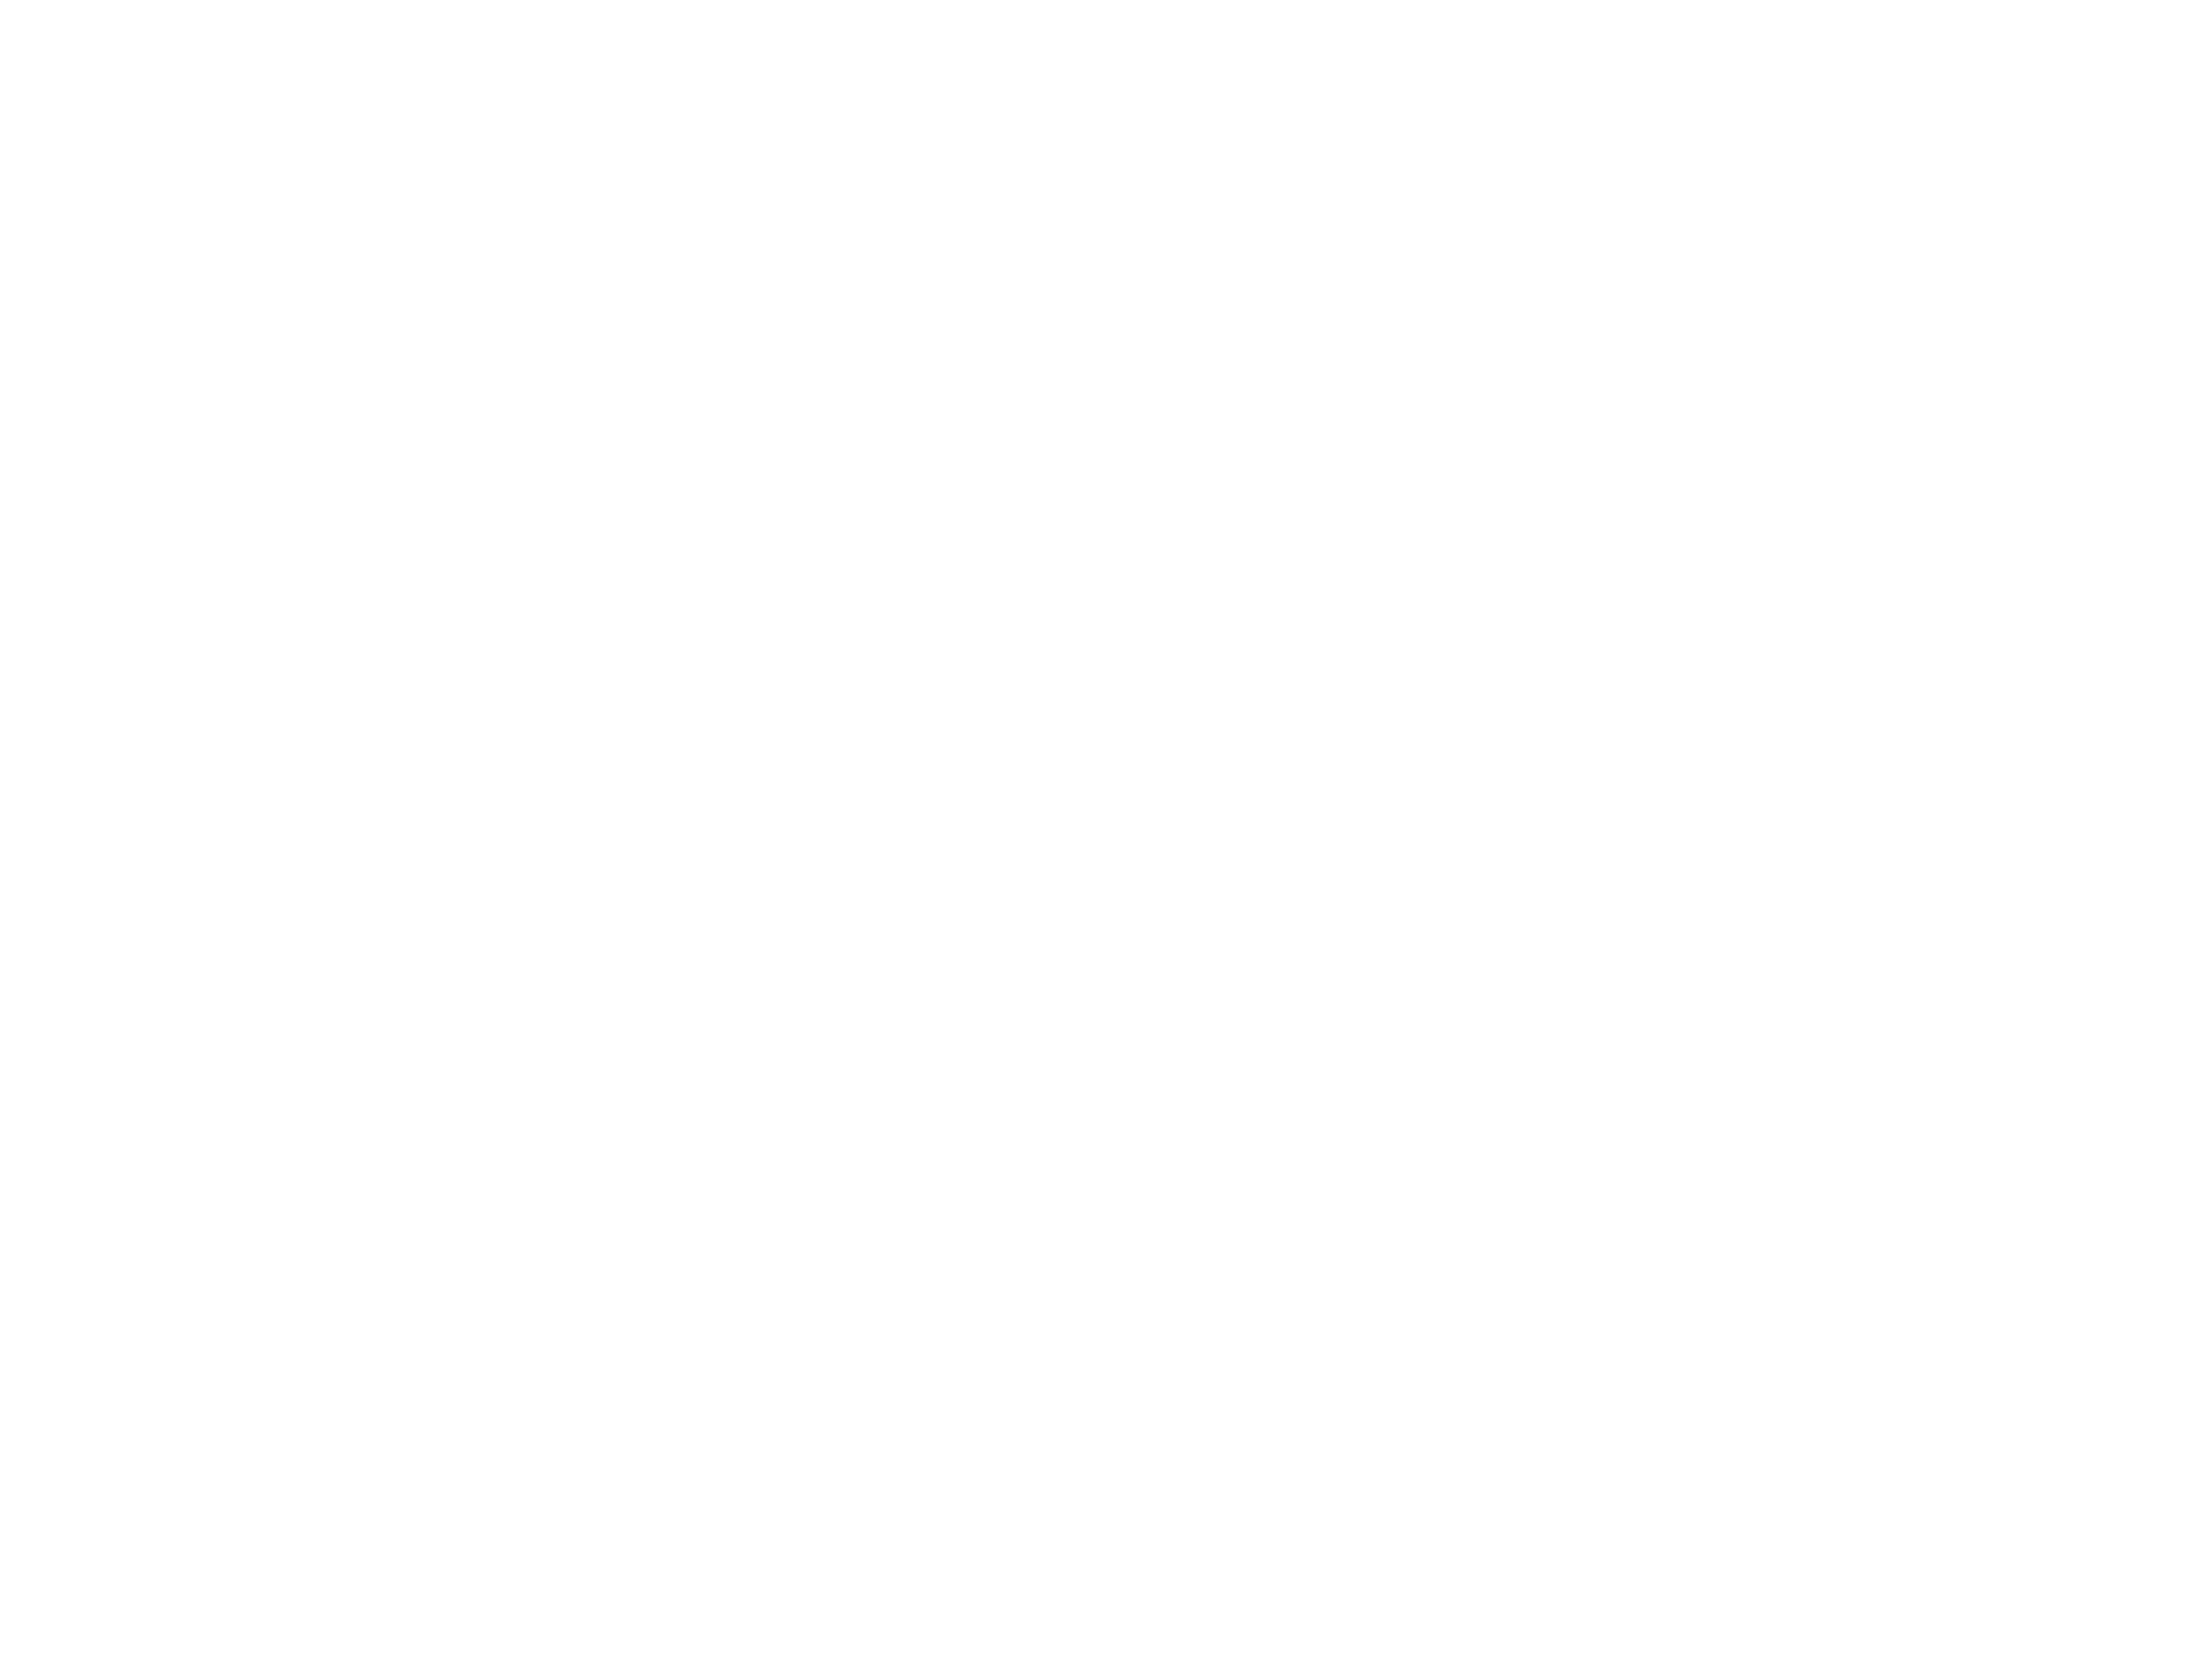
\includegraphics[scale=0.8]{graph/aim7}
\end{frame}

\begin{frame}{AIM7}
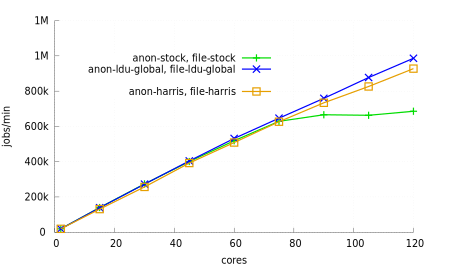
\includegraphics[scale=0.8]{graph/aim7_1}
\end{frame}

\begin{frame}{AIM7}
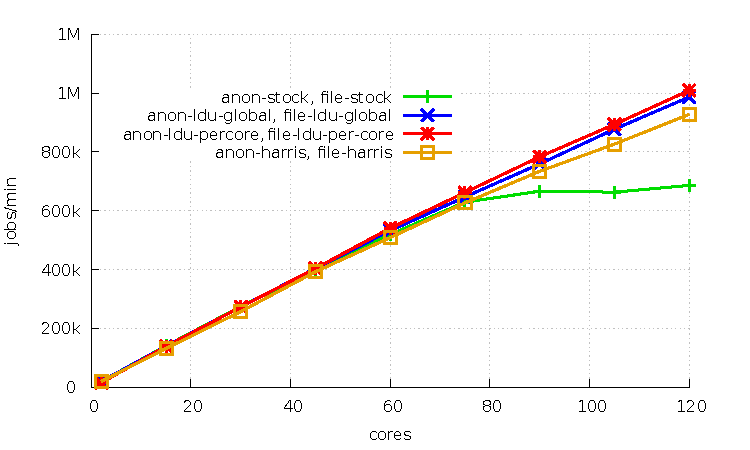
\includegraphics[scale=0.8]{graph/aim7_2}
\end{frame}


\begin{frame}{AIM7 - CPU utilization}
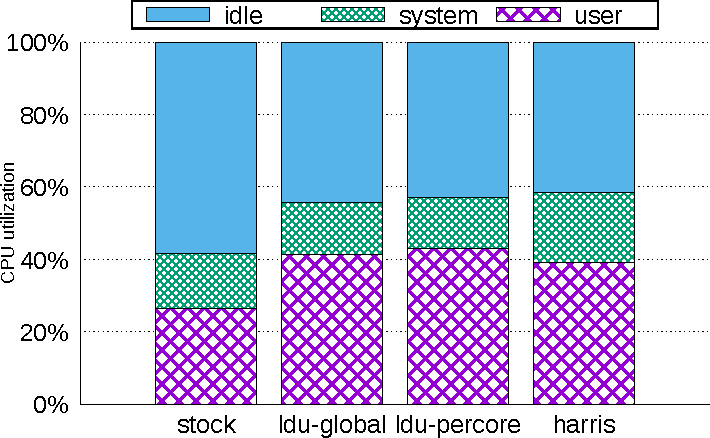
\includegraphics[scale=0.8]{graph/aim7_cpuutils}
\end{frame}

\begin{frame}{EXIM}
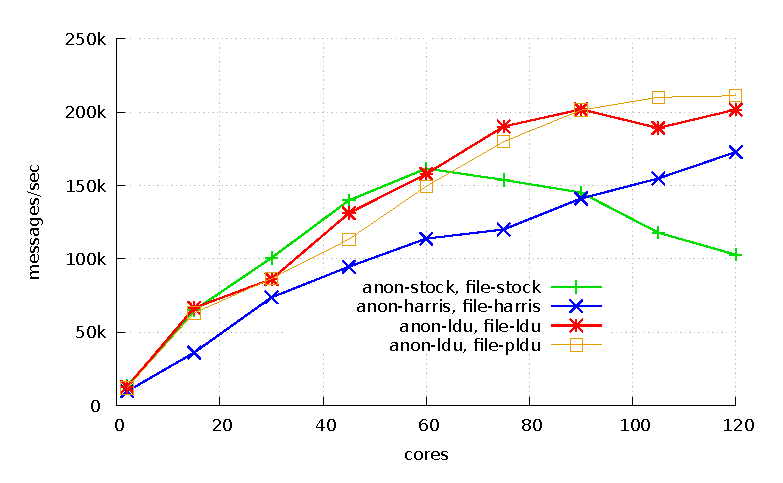
\includegraphics[scale=0.8]{graph/exim}
\end{frame}


\begin{frame}{EXIM - CPU utilization}
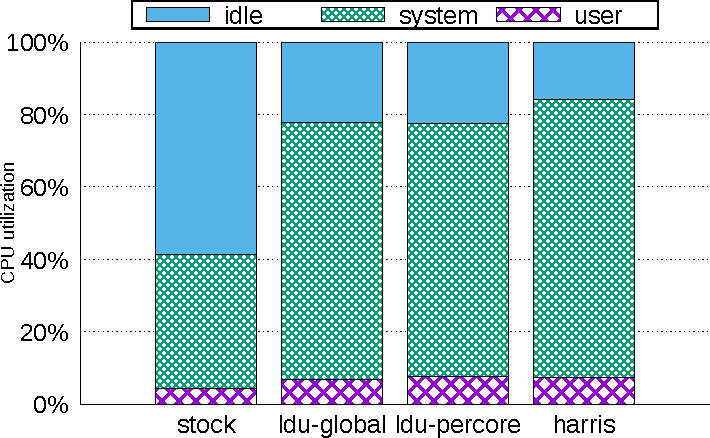
\includegraphics[scale=0.8]{graph/exim_cpuutils}
\end{frame}


\begin{frame}{Lmbench}
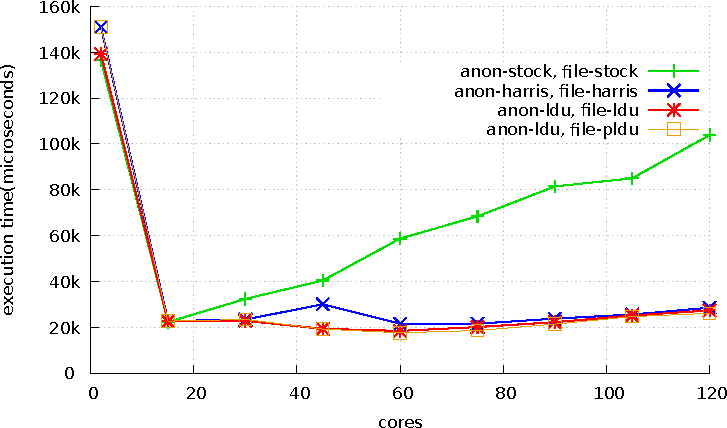
\includegraphics[scale=0.8]{graph/lmbench}
\end{frame}


\begin{frame}{Lmbench - CPU utilization}
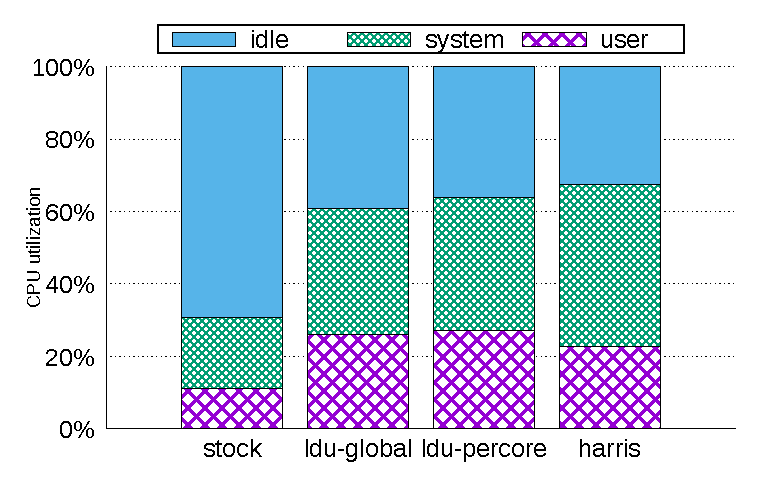
\includegraphics[scale=0.8]{graph/lmbench_cpuutils}
\end{frame}


\begin{frame}{Update ratios - AIM7}
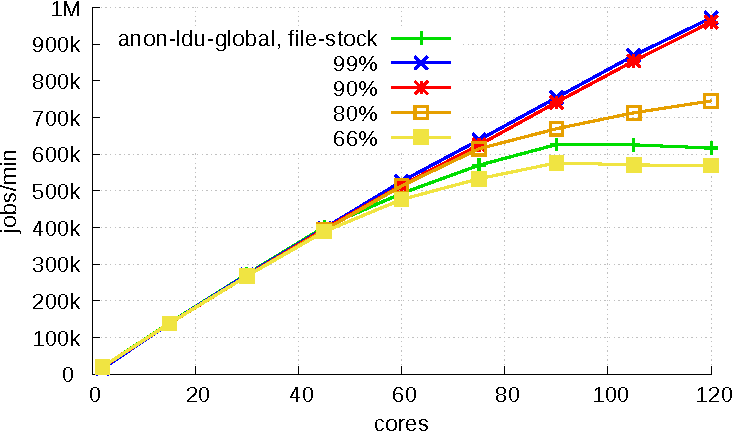
\includegraphics[scale=0.4]{graph/ratio_aim7_core}
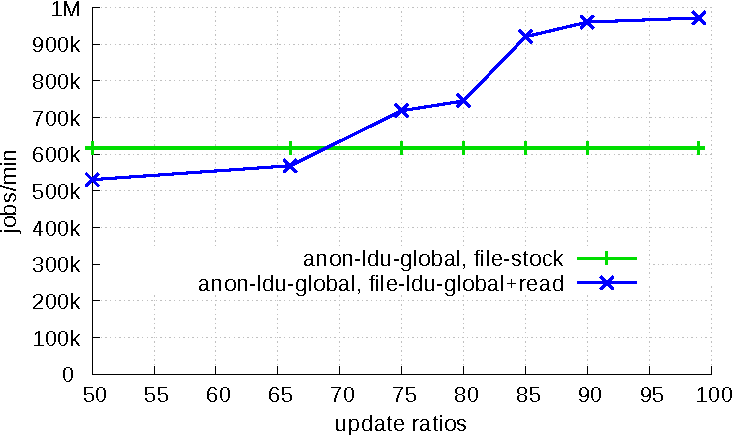
\includegraphics[scale=0.4]{graph/ratio_aim7}
\end{frame}

\begin{frame}{Update ratios - Exim}
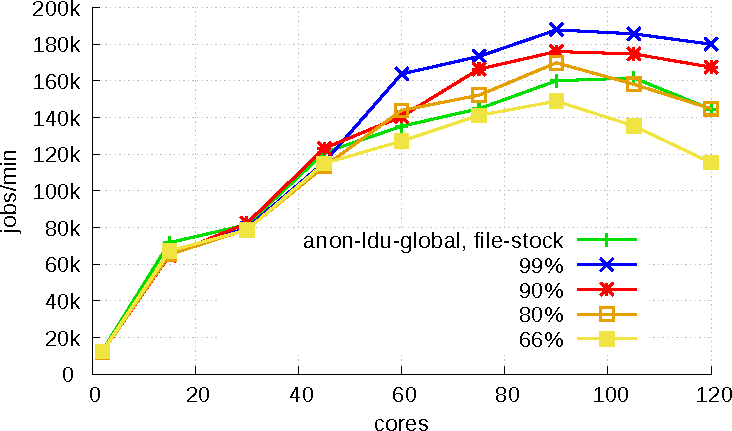
\includegraphics[scale=0.4]{graph/ratio_exim_core}
\includegraphics[scale=0.4]{graph/ratio_exim}
\end{frame}

\begin{frame}{Update ratios - Lmbench}
\includegraphics[scale=0.4]{graph/ratio_lmbench_core}
\includegraphics[scale=0.4]{graph/ratio_lmbench}
\end{frame}


\begin{frame}{Related work}
\begin{itemize}
    \item Operating systems scalability.
    \begin{itemize}
    \item Create new operating systems.
    \item Optimize existing operating systems.
    \end{itemize}    
    \item Scalable lock.
    \begin{itemize}
    \item Queue-based locks.
    \item Hierarchical locks.
    \item Delegation techniques.
    \end{itemize}
    \item Scalable data structures.
    \begin{itemize}
    \item Different performances depending on their update ratios.
    \end{itemize}
    \end{itemize}
\end{frame}


%\begin{frame}{Curriculum Vitae}
%\includegraphics[scale=0.5]{cv/cv0}
%\end{frame}

%\begin{frame}{Curriculum Vitae}
%\includegraphics[scale=0.5]{cv/cv1}
%\end{frame}

%\begin{frame}{Curriculum Vitae}
%\includegraphics[scale=0.5]{cv/cv2}
%\end{frame}

\begin{frame}{Futuer Directions}
	\begin{itemize} 
	\item Combine LDU with time-stamp based approach for stack, queue.
	\item Combine RCU readers with log-based updates.
	\end{itemize}
\end{frame}

\begin{frame}{Combine RCU readers with log-based updates}
\includegraphics[scale=0.5]{fig/log-based}
\end{frame}


\begin{frame}{Conclusion}
    \begin{itemize}
    \item \text{https://github.com/manycore-ldu/ldu}
    \end{itemize}
\end{frame}


\end{document}
